% Options for packages loaded elsewhere
\PassOptionsToPackage{unicode}{hyperref}
\PassOptionsToPackage{hyphens}{url}
%
\documentclass[
]{article}
\usepackage{amsmath,amssymb}
\usepackage{iftex}
\ifPDFTeX
  \usepackage[T1]{fontenc}
  \usepackage[utf8]{inputenc}
  \usepackage{textcomp} % provide euro and other symbols
\else % if luatex or xetex
  \usepackage{unicode-math} % this also loads fontspec
  \defaultfontfeatures{Scale=MatchLowercase}
  \defaultfontfeatures[\rmfamily]{Ligatures=TeX,Scale=1}
\fi
\usepackage{lmodern}
\ifPDFTeX\else
  % xetex/luatex font selection
\fi
% Use upquote if available, for straight quotes in verbatim environments
\IfFileExists{upquote.sty}{\usepackage{upquote}}{}
\IfFileExists{microtype.sty}{% use microtype if available
  \usepackage[]{microtype}
  \UseMicrotypeSet[protrusion]{basicmath} % disable protrusion for tt fonts
}{}
\makeatletter
\@ifundefined{KOMAClassName}{% if non-KOMA class
  \IfFileExists{parskip.sty}{%
    \usepackage{parskip}
  }{% else
    \setlength{\parindent}{0pt}
    \setlength{\parskip}{6pt plus 2pt minus 1pt}}
}{% if KOMA class
  \KOMAoptions{parskip=half}}
\makeatother
\usepackage{xcolor}
\usepackage[margin=1in]{geometry}
\usepackage{color}
\usepackage{fancyvrb}
\newcommand{\VerbBar}{|}
\newcommand{\VERB}{\Verb[commandchars=\\\{\}]}
\DefineVerbatimEnvironment{Highlighting}{Verbatim}{commandchars=\\\{\}}
% Add ',fontsize=\small' for more characters per line
\usepackage{framed}
\definecolor{shadecolor}{RGB}{248,248,248}
\newenvironment{Shaded}{\begin{snugshade}}{\end{snugshade}}
\newcommand{\AlertTok}[1]{\textcolor[rgb]{0.94,0.16,0.16}{#1}}
\newcommand{\AnnotationTok}[1]{\textcolor[rgb]{0.56,0.35,0.01}{\textbf{\textit{#1}}}}
\newcommand{\AttributeTok}[1]{\textcolor[rgb]{0.13,0.29,0.53}{#1}}
\newcommand{\BaseNTok}[1]{\textcolor[rgb]{0.00,0.00,0.81}{#1}}
\newcommand{\BuiltInTok}[1]{#1}
\newcommand{\CharTok}[1]{\textcolor[rgb]{0.31,0.60,0.02}{#1}}
\newcommand{\CommentTok}[1]{\textcolor[rgb]{0.56,0.35,0.01}{\textit{#1}}}
\newcommand{\CommentVarTok}[1]{\textcolor[rgb]{0.56,0.35,0.01}{\textbf{\textit{#1}}}}
\newcommand{\ConstantTok}[1]{\textcolor[rgb]{0.56,0.35,0.01}{#1}}
\newcommand{\ControlFlowTok}[1]{\textcolor[rgb]{0.13,0.29,0.53}{\textbf{#1}}}
\newcommand{\DataTypeTok}[1]{\textcolor[rgb]{0.13,0.29,0.53}{#1}}
\newcommand{\DecValTok}[1]{\textcolor[rgb]{0.00,0.00,0.81}{#1}}
\newcommand{\DocumentationTok}[1]{\textcolor[rgb]{0.56,0.35,0.01}{\textbf{\textit{#1}}}}
\newcommand{\ErrorTok}[1]{\textcolor[rgb]{0.64,0.00,0.00}{\textbf{#1}}}
\newcommand{\ExtensionTok}[1]{#1}
\newcommand{\FloatTok}[1]{\textcolor[rgb]{0.00,0.00,0.81}{#1}}
\newcommand{\FunctionTok}[1]{\textcolor[rgb]{0.13,0.29,0.53}{\textbf{#1}}}
\newcommand{\ImportTok}[1]{#1}
\newcommand{\InformationTok}[1]{\textcolor[rgb]{0.56,0.35,0.01}{\textbf{\textit{#1}}}}
\newcommand{\KeywordTok}[1]{\textcolor[rgb]{0.13,0.29,0.53}{\textbf{#1}}}
\newcommand{\NormalTok}[1]{#1}
\newcommand{\OperatorTok}[1]{\textcolor[rgb]{0.81,0.36,0.00}{\textbf{#1}}}
\newcommand{\OtherTok}[1]{\textcolor[rgb]{0.56,0.35,0.01}{#1}}
\newcommand{\PreprocessorTok}[1]{\textcolor[rgb]{0.56,0.35,0.01}{\textit{#1}}}
\newcommand{\RegionMarkerTok}[1]{#1}
\newcommand{\SpecialCharTok}[1]{\textcolor[rgb]{0.81,0.36,0.00}{\textbf{#1}}}
\newcommand{\SpecialStringTok}[1]{\textcolor[rgb]{0.31,0.60,0.02}{#1}}
\newcommand{\StringTok}[1]{\textcolor[rgb]{0.31,0.60,0.02}{#1}}
\newcommand{\VariableTok}[1]{\textcolor[rgb]{0.00,0.00,0.00}{#1}}
\newcommand{\VerbatimStringTok}[1]{\textcolor[rgb]{0.31,0.60,0.02}{#1}}
\newcommand{\WarningTok}[1]{\textcolor[rgb]{0.56,0.35,0.01}{\textbf{\textit{#1}}}}
\usepackage{longtable,booktabs,array}
\usepackage{calc} % for calculating minipage widths
% Correct order of tables after \paragraph or \subparagraph
\usepackage{etoolbox}
\makeatletter
\patchcmd\longtable{\par}{\if@noskipsec\mbox{}\fi\par}{}{}
\makeatother
% Allow footnotes in longtable head/foot
\IfFileExists{footnotehyper.sty}{\usepackage{footnotehyper}}{\usepackage{footnote}}
\makesavenoteenv{longtable}
\usepackage{graphicx}
\makeatletter
\newsavebox\pandoc@box
\newcommand*\pandocbounded[1]{% scales image to fit in text height/width
  \sbox\pandoc@box{#1}%
  \Gscale@div\@tempa{\textheight}{\dimexpr\ht\pandoc@box+\dp\pandoc@box\relax}%
  \Gscale@div\@tempb{\linewidth}{\wd\pandoc@box}%
  \ifdim\@tempb\p@<\@tempa\p@\let\@tempa\@tempb\fi% select the smaller of both
  \ifdim\@tempa\p@<\p@\scalebox{\@tempa}{\usebox\pandoc@box}%
  \else\usebox{\pandoc@box}%
  \fi%
}
% Set default figure placement to htbp
\def\fps@figure{htbp}
\makeatother
\setlength{\emergencystretch}{3em} % prevent overfull lines
\providecommand{\tightlist}{%
  \setlength{\itemsep}{0pt}\setlength{\parskip}{0pt}}
\setcounter{secnumdepth}{-\maxdimen} % remove section numbering
\usepackage{booktabs}
\usepackage{longtable}
\usepackage{array}
\usepackage{multirow}
\usepackage{wrapfig}
\usepackage{float}
\usepackage{colortbl}
\usepackage{pdflscape}
\usepackage{tabu}
\usepackage{threeparttable}
\usepackage{threeparttablex}
\usepackage[normalem]{ulem}
\usepackage{makecell}
\usepackage{xcolor}
\usepackage{siunitx}

    \newcolumntype{d}{S[
      table-align-text-before=false,
      table-align-text-after=false,
      input-symbols={-,\*+()}
    ]}
  
\usepackage{bookmark}
\IfFileExists{xurl.sty}{\usepackage{xurl}}{} % add URL line breaks if available
\urlstyle{same}
\hypersetup{
  pdftitle={Data Scoping: Job Search Behaviour},
  pdfauthor={Ebba Mark},
  hidelinks,
  pdfcreator={LaTeX via pandoc}}

\title{Data Scoping: Job Search Behaviour}
\author{Ebba Mark}
\date{2025-07-30}

\begin{document}
\maketitle

\section{Overview}\label{overview}

The following document summarises current progress on identifying data
sources to inform the job search behaviour in our labour market ABM.

\textbf{Goals:}

\begin{enumerate}
\def\labelenumi{\arabic{enumi}.}
\item
  Identify parameters relevant to agent search behaviour in the ABM.
\item
  Assess data quality for deriving empirical estimates of these
  parameters.
\end{enumerate}

We have narrowed the list of behavioural adjustments to the following:\\
- \textbf{Duration-dependent search effort}\\
- \textbf{Reservation Wage Adjustment Rates}\\
- \textbf{Cyclical On-the-Job Search}\\
- \textbf{Risk Aversion}: For now this is randomised to ensure variation
in vacancy targeting by similar workers. This is not yet supported by
data.

\section{Calibrating Behavioural
Mechanisms}\label{calibrating-behavioural-mechanisms}

\textbf{Data we have decided to keep:}

\begin{enumerate}
\def\labelenumi{\arabic{enumi}.}
\item
  Current Population Survey 2018 \& 2022: Information on applications
  sent by unemployment duration.
\item
  Displaced Worker Supplement: As part of the Current Population Survey,
  the US Census Bureau conducts an annual Displaced Worker Supplement in
  which workers who have lost their job in the last three years are
  asked additional questions about their unemployment experiences and
  (if re-employed) their re-employment conditions. From this we draw a
  reservation wage adjustment rate as a function of unemployment
  duration.
\item
  \href{https://www.aeaweb.org/articles?id=10.1257/mac.20180105}{Eeckhout
  et al.~2019 Unemployment Cycles}: We derive the sensitivity of
  employed job seekers to the business cycle from the
  employment-to-employment transitions data as used in Eeckhout et
  al.~Due to unreliable component parts of the Eeckhout analysis, we
  decided to abandon using their estimated parameters (search intensity
  for employed workers).
\item
  (Validation) Mukoyama et al.~data on the intensive margin of
  unemployed search effort (in minutes searched) over the business
  cycle. We have chosen to include this as a validation exercise of our
  application effort imposition.
\item
  \href{https://www.aeaweb.org/articles?id=10.1257/aer.20190808}{\textbf{Mueller
  et al.~2021: Job Seekers' Perceptions and Employment Prospects:
  Heterogeneity, Duration Dependence and Bias}}
\end{enumerate}

\textbf{Additional analyses that we have decided to exclude as data
inputs due to lack of relevance or poor data quality are in the
``Discarded Analyses'' tab.}

\subsection{Applications Sent}\label{applications-sent}

\subsubsection{(Calibration) Current Population Survey - 2018 \& 2020
Supplement}\label{calibration-current-population-survey---2018-2020-supplement}

This 2020
\href{https://www.bls.gov/opub/btn/volume-9/how-do-jobseekers-search-for-jobs.htm\#_edn5}{``Beyond
the Numbers'' issue} distills insights from a 2018 Supplement to the
Current Population Survey. The below plots show the highlights relevant
to our decision-making on the job search process. In nearly all cases,
the results are ``binned'' into intervals (ie. number of people sending
81 or more applications or unemployment duration of between 5 and 14
weeks) which means that any line plots (or linear interpretation of the
bar graph) should be done carefully. Preliminary results using the raw
data are found in the next section.

\begin{itemize}
\item
  Figure 1: Shows the proportion of all individuals sending x amount of
  applications receiving y amount of interviews. The plot indicates a
  ``consistent'' return to sending more applications, although as
  demonstrated in Figure 3, the number of interviews received does not
  necessarily equate to receiving a job offer.
\item
  Figure 2: Demonstrates the number of applications sent (red),
  interviews received (green), average interview:applicaiton ratio
  (blue), and probability of receiving a job offer (purple) by
  individuals in each category of unemployment duration. There is some
  indication (although, again, interpretation is difficult without the
  raw data) that both effort and success seems to increase and then
  decline with time spent in unemployment, apart from success as
  measured by receiving a job offer which seems to consistently decline
  with time spent in unemployment.
\item
  Figure 3: Percentage of jobseekers receiving an offer seems to
  increase as a function of the number of applications sent, until a
  certain point.
\end{itemize}

\begin{verbatim}
## Processing URL: https://www.bls.gov/opub/btn/volume-9/how-do-jobseekers-search-for-jobs.htm#_edn2
\end{verbatim}

\pandocbounded{\includegraphics[keepaspectratio]{behav_params_overview_files/figure-latex/unnamed-chunk-1-1.pdf}}

\begin{verbatim}
## NULL
\end{verbatim}

It turns out that the 2018 supplement was also run in 2022, giving us
two sets of years to compare (including pre- and post-Covid). The below
looks at the
\href{https://www.census.gov/data/datasets/time-series/demo/cps/cps-supp_cps-repwgt/cps-unemployment.2022.html\#list-tab-1269561637}{raw
data} that underlies the plotting immediately above, plus the additional
data from 2022. Below find a preliminary scatter plot of applications
sent versus unemployment duration. Each individual is asked how many
applications they sent in the last two months (two-month periods are
indicated by the grey gridlines, for reference). This does NOT include
data in on the job search.

\textbf{Data Source:} Unemployment Insurance Nonfilers Supplement
conducted in 2018 (n = 3,268) \& 2022 (n = 1,901) where individuals who
are unemployed but have not filed for unemployment insurance are asked
the following:

\begin{figure}
\centering
\pandocbounded{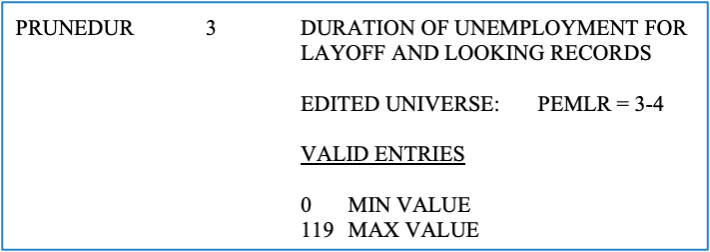
\includegraphics[keepaspectratio]{CPS_BLS_Supplement_18_22/udur_survey_question.png}}
\caption{Survey Question: Unemployment Duration}
\end{figure}

\begin{figure}
\centering
\pandocbounded{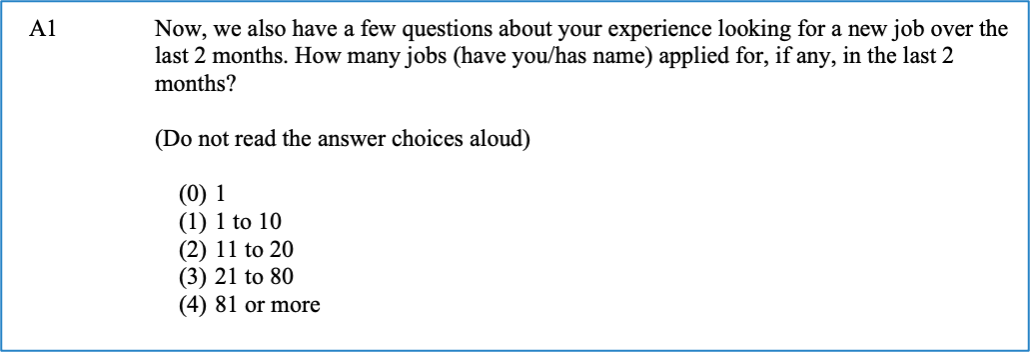
\includegraphics[keepaspectratio]{CPS_BLS_Supplement_18_22/apps_sent_question.png}}
\caption{Survey Question: Applications Sent}
\end{figure}

\pandocbounded{\includegraphics[keepaspectratio]{behav_params_overview_files/figure-latex/unnamed-chunk-2-1.pdf}}

Below, I display the results of an exploration of the probability of
reporting a specific number of applications sent (in the bins as in the
survey question above) using various specifications of an ordinal
logistic regression. I test specifications varying three different model
parameters: 1. link function\\
2. linear vs.~quadratic unemploymentduration,\\
3. with and without demographic control variables (education, gender,
age, family income - race excluded because of lack of statistical
significance though this can be revisited.)

We estimate an ordinal logistic regression model for reported
applications sent \(Y_i in {0, 1, 2, 3, 4}\) testing four different link
functions: the complementary log-log (cloglog), logistic, log-log, and
probit link functions. Let \(X_i^\top \beta\) denote the predictor
variable. The cumulative probability of observing response category
\(j\) or below, \(\Pr(Y_i \leq j \mid X_i)\), is modeled as follows for
each link function:

\begin{align*}
\text{Complementary log-log (cloglog):} \quad & \Pr(Y_i \leq j \mid X_i) = 1 - \exp\left( -\exp\left( \tau_j - X_i^\top \beta \right) \right) \\
\text{Logistic (logit):} \quad & \Pr(Y_i \leq j \mid X_i) = \frac{1}{1 + \exp\left( -(\tau_j - X_i^\top \beta) \right)} \\
\text{Loglog:} \quad & \Pr(Y_i \leq j \mid X_i) = \exp\left( -\exp\left( -(\tau_j - X_i^\top \beta) \right) \right) \\
\text{Probit:} \quad & \Pr(Y_i \leq j \mid X_i) = \Phi(\tau_j - X_i^\top \beta)
\end{align*}

Here, \(\Phi(\cdot)\) denotes the cumulative distribution function of
the standard normal distribution. The estimated coefficients \(\beta\)
are interpreted conditional on the choice of link function where \(X_i\)
is either:

\(X_i = \left( \text{Unemp.Dur.}_i \right)\)

\(X_i = \left( \text{Unemp.Dur.}_i^2 \right)\)

\(X_i = \left( \text{Unemp.Dur.}_i, \text{Unemp.Dur.}_i^2 \right)\)

with and without control variables (education, gender, age, family
income).

Assumptions about the probability distribution of the errors associated
with each link function:\\
- \emph{Logit:} good when the response behavior is symmetric around the
middle category.\\
- \emph{Probit:} When you're assuming a normal latent error distribution
or want closer fit to Gaussian processes.\\
- \emph{Complementary log-log:} When the likelihood of being in a higher
category increases sharply but asymmetrically, or you expect hazard-like
dynamics.\\
- \emph{Log-log:} When early categories are of more importance and need
sharper separation.

\emph{Preliminary hypothesis:} Best fit will be with a complementary
log-log as we care more about distinguishing between lower-level bins
and there are few observations in the highest-level bins.

\pandocbounded{\includegraphics[keepaspectratio]{behav_params_overview_files/figure-latex/unnamed-chunk-3-1.pdf}}
\pandocbounded{\includegraphics[keepaspectratio]{behav_params_overview_files/figure-latex/unnamed-chunk-3-2.pdf}}
\pandocbounded{\includegraphics[keepaspectratio]{behav_params_overview_files/figure-latex/unnamed-chunk-3-3.pdf}}

Using an AIC information criterion to compare the fit across all models,
the following results are clear:\\
1. Models with control variables consistently perform better than those
without.\\
2. Looking at the plots above, the relationship between unemployment
duration and the predicted probability of reporting each application
effort bin is very consistent except in the case of the log-log link
function (blue in the panels above). In the plot below comparing the AIC
the log-log link function (represented by the square symbol below) is
consistently worse than all other link functions. This indicates
consistency in the results reported above. Intuitively, the log-log link
function is likely to be an unreasonable fit for the latent variable as
we care more about shifts in the lower-level categories than
higher-level categories.\\
3. A complementary log-log specification for the latent variable is most
suitable. This follows logically from the fact that the probability of
being in the highest-level categories is relatively low.\\
4. Finally, a specification with a linear and quadratic estimator is
consistently better than either the specification with simply a linear
OR quadratic unemployment duration estimator indicating that the
probability distributions represented in the final panel above are
likely to be the best fit.

\emph{Result:} For each additional quarter of unemployment, an
individual's odds of dropping to a lower-level application category
decreases by \textasciitilde.1\%. This is statistically significant
across all specifications at the 0.1\% level.

\pandocbounded{\includegraphics[keepaspectratio]{behav_params_overview_files/figure-latex/unnamed-chunk-4-1.pdf}}

\begin{verbatim}
## [1] TRUE
\end{verbatim}

\begin{verbatim}
## [1] TRUE
\end{verbatim}

\pandocbounded{\includegraphics[keepaspectratio]{behav_params_overview_files/figure-latex/unnamed-chunk-5-1.pdf}}

\subsubsection{(Validation) Mukoyama et al.~Job Search and the Business
Cycle}\label{validation-mukoyama-et-al.-job-search-and-the-business-cycle}

\href{https://www.aeaweb.org/articles?id=10.1257/mac.20160202}{Mukoyama:
Job Search Over the Business Cycle}

\pandocbounded{\includegraphics[keepaspectratio]{behav_params_overview_files/figure-latex/unnamed-chunk-6-1.pdf}}
\pandocbounded{\includegraphics[keepaspectratio]{behav_params_overview_files/figure-latex/unnamed-chunk-6-2.pdf}}
\pandocbounded{\includegraphics[keepaspectratio]{behav_params_overview_files/figure-latex/unnamed-chunk-6-3.pdf}}
\pandocbounded{\includegraphics[keepaspectratio]{behav_params_overview_files/figure-latex/unnamed-chunk-6-4.pdf}}

\subsection{Reservation Wage
Adjustment}\label{reservation-wage-adjustment}

As part of the Current Population Survey, the US Census Bureau conducts
an annuaol
\href{https://cps.ipums.org/cps/dw_sample_notes.shtml}{Displaced Worker
Supplement} in which workers who have lost their job in the last three
years are asked additional questions about their unemployment
experiences and (if re-employed) their re-employment conditions.

``The universe for the Displaced Workers Supplement is civilians 20 or
older. Respondents are further categorized as a''displaced worker'' if
they meet additional characteristics (see DWSTAT). After 1998, displaced
workers are those who lost or left a job due to layoffs or shutdowns
within the past 3 years\ldots were not self-employed, and did not expect
to be recalled to work within the next six months.

The data used below is from annual survey responses between 2000-2025. I
use the supplement sample weights in all results below. I note where I
have clipped the sample for outliers (wage ratio between {[}0.25, 2{]}
and unemployment duration less than 96 weeks (\textasciitilde24 months).

Below I:

\begin{enumerate}
\def\labelenumi{\arabic{enumi}.}
\tightlist
\item
  \textbf{Data Cleaning Procedure:} Show data cleaning just for
  reference (feel free to ignore)!.
\item
  \textbf{Descriptives:} Show some descriptives about the data itself.
\item
  \textbf{Regression Results on Non-Uniform Sample:} Regression results
  with ratio of new wage to wage at the lost job (\(W_{h}\) and
  \(W_{w}\)) regressed (cross-sectionally) on unemployment duration with
  and without various combinations of control variables (whether or not
  an individual received unemployment compensation, age, race, sex,
  marital status, education, previous wage level. ) Note that the wages
  are reported in hourly and weekly values but. this reporting is
  inconsistent across observations. In other words, though most
  individuals (4600/6198) report their wage in both units, 270 report
  only hourly and 1328 report only weekly. I have not reconciled the
  inconsistency so I use hourly wage ratios in majority of the below
  document. I could try to reconcile this.
\item
  Outline some considerations for further improvement of the analysis:

  \begin{enumerate}
  \def\labelenumii{\arabic{enumii}.}
  \tightlist
  \item
    \textbf{Reweighted Samples:} The sample is non-uniform in
    unemployment duration (less observations as unemployment duration
    increases). Try two methods of reweighting to address selection
    issues (Heckman Selection correction - though I think this is
    inappropriate for this particular selection issue) and non-uniform
    (entropy-balancing to deal with representativeness of population
    over unemployment durations) sample confirm regression results in
    non-uniform sample.
  \item
    \textbf{Representativeness of the Sample (Education, Age, Gender,
    and Wage):} Representativeness of the data to motivate data
    limitations and inform the ultimate reweighting scheme.
  \end{enumerate}
\end{enumerate}

\textbf{Overall result (at the moment):} Individuals accept a
\textasciitilde1-percentage point change in the wage ratio per
additional month of unemployment. Variations using model reweighting,
different samples, combinations of control variables, reported hourly
and weekly wage ratios do not seem to affect the result. However, the
data seems to follow a non-linear relationship (we see little
satisficing until around \textasciitilde12 months of unemployment) after
which the wage ratio begins to decrease. Individuals seem to accept a
below-1 relative wage ratio (current wage:wage at lost job) following a
year of unemployment. If we fit this model with a quadratic fit this
could inform our reservation wage adjustment parameter in the model.

\textbf{Important Considerations/Limitations:}

\begin{enumerate}
\def\labelenumi{\arabic{enumi}.}
\tightlist
\item
  \textbf{Displaced worker classification as outlined above.} Can we
  generalise from this definition to all unemployed workers?
\item
  \textbf{The reported `current wage' is not necessarily the the
  realised wage post-re-employment.} Individuals report the wage at the
  lost job, the amount of time unemployed until they were re-employed,
  and the wage they hold at their current job. However, it is not
  indicated whether the current job is the same job as the first they
  were re-employed at. Given various comments in the literature about
  finding ``stop-gap'' employment, this might not be a problem in the
  sense that the ``current wage'' would more accurately indicate the
  wage an individual has ``landed'' at post-unemployment spell. But
  curious what you think about the defensibility of this.
\item
  \textbf{Outcome variable:} How do we feel about the outcome variable
  as the ratio of current to latest held job? Might we want to take the
  log or consider simply the (log) level regressed on the previous wage.
  Wondering if a ratio-based outcome variable might muddle
  interpretation. Curious for your reactions.
\end{enumerate}

\subsection{Data cleaning}\label{data-cleaning}

Feel free to ignore this code chunk immediately below - included for now
for transparency in case you spot issues. I include it for your info on
binning and outlier trimming.

\begin{Shaded}
\begin{Highlighting}[]
\CommentTok{\# From the original dataset, I include only those that reported having lost a }
\CommentTok{\# FT job in the last three years}
\NormalTok{df }\OtherTok{\textless{}{-}} \FunctionTok{readRDS}\NormalTok{(}\FunctionTok{here}\NormalTok{(}\StringTok{"data/behav\_params/cps\_displaced\_worker\_supplement/cps\_disp\_filtered.RDS"}\NormalTok{)) }\SpecialCharTok{\%\textgreater{}\%} 
  \FunctionTok{select}\NormalTok{(hwtfinl, cpsid, wtfinl, age, sex, race, marst, educ, }
         \CommentTok{\# age, sex, race, marital status, educational attainment}
\NormalTok{         dwsuppwt, }\CommentTok{\# Survey weight}
\NormalTok{         dwyears, }\CommentTok{\# Years worked at lost job}
\NormalTok{         dwben, }\CommentTok{\# Received unemployment benefits}
\NormalTok{         dwexben, }\CommentTok{\# Exhausted unemployment benefits}
\NormalTok{         dwlastwrk, }\CommentTok{\# Time since worked at last job}
\NormalTok{         dwweekc, }\CommentTok{\# Weekly earnings at current job}
\NormalTok{         dwweekl, }\CommentTok{\# Weekly earnings at lost job}
\NormalTok{         dwwagel, }\CommentTok{\# Hourly earnings at lost job}
\NormalTok{         dwwagec, }\CommentTok{\# Hourly wage at current job}
\NormalTok{         dwhrswkc, }\CommentTok{\# Hours worked each week at current job}
\NormalTok{         dwresp, }\CommentTok{\# Eligibility and interview status for Displaced Wrkr Supplement}
         \CommentTok{\# Interestingly the unemployment duration is not directly linked to }
         \CommentTok{\# CURRENT job and we cannot see the wage of the start of the next job...}
        \CommentTok{\# thought this feels problematic, it does indicate more accurately the }
        \CommentTok{\# ultimate "recovered" wage...will need to declare as a limitation }
        \CommentTok{\# but also not completely indefensible}
\NormalTok{         dwwksun) }\SpecialCharTok{\%\textgreater{}\%}  \CommentTok{\# Number of weeks not working between between end of lost}
         \CommentTok{\# or left job and start of next job}
  \CommentTok{\# I remove anyone who is Not in Universe (99) and declaring greater than 160 }
  \CommentTok{\# weeks unemployed between jobs}
\FunctionTok{filter}\NormalTok{(dwhrswkc }\SpecialCharTok{!=} \DecValTok{99} \SpecialCharTok{\&}\NormalTok{ dwwksun }\SpecialCharTok{\textless{}=} \DecValTok{160}\NormalTok{) }\SpecialCharTok{\%\textgreater{}\%} 
  \CommentTok{\# Replacing NIU values with NA values}
  \FunctionTok{mutate}\NormalTok{(}\AttributeTok{dwwagel =} \FunctionTok{ifelse}\NormalTok{(}\FunctionTok{round}\NormalTok{(dwwagel) }\SpecialCharTok{==} \DecValTok{100}\NormalTok{, }\ConstantTok{NA}\NormalTok{, dwwagel),}
         \AttributeTok{dwwagec =} \FunctionTok{ifelse}\NormalTok{(}\FunctionTok{round}\NormalTok{(dwwagec) }\SpecialCharTok{==} \DecValTok{100}\NormalTok{, }\ConstantTok{NA}\NormalTok{, dwwagec),}
         \AttributeTok{dwweekl =} \FunctionTok{ifelse}\NormalTok{(}\FunctionTok{round}\NormalTok{(dwweekl) }\SpecialCharTok{==} \DecValTok{10000}\NormalTok{, }\ConstantTok{NA}\NormalTok{, dwweekl),}
         \AttributeTok{dwweekc =} \FunctionTok{ifelse}\NormalTok{(}\FunctionTok{round}\NormalTok{(dwweekc) }\SpecialCharTok{==} \DecValTok{10000}\NormalTok{, }\ConstantTok{NA}\NormalTok{, dwweekc),}
         \CommentTok{\# dwwage\_rec\_l = ifelse(is.na(dwagel) \& !is.na(dweekl) \textasciitilde{} dwweekl),}
         \CommentTok{\# dwweekc = ifelse(round(dwweekc) == 10000, NA, dwweekc),}
         \CommentTok{\# Binning educational categories}
         \AttributeTok{educ\_cat =} \FunctionTok{factor}\NormalTok{(}\FunctionTok{case\_when}\NormalTok{(educ }\SpecialCharTok{\%in\%} \FunctionTok{c}\NormalTok{(}\DecValTok{1}\NormalTok{) }\SpecialCharTok{\textasciitilde{}} \ConstantTok{NA}\NormalTok{, }\CommentTok{\# (NIU)}
\NormalTok{                              educ }\SpecialCharTok{\textgreater{}} \DecValTok{1} \SpecialCharTok{\&}\NormalTok{ educ }\SpecialCharTok{\textless{}=} \DecValTok{71} \SpecialCharTok{\textasciitilde{}} \StringTok{"Less than HS"}\NormalTok{, }\CommentTok{\# Includes }
                                  \CommentTok{\# "None" {-} Grade 12 no diploma }
                                  \CommentTok{\# (8 subcategories (grade 1{-}11 etc))}
\NormalTok{                              educ }\SpecialCharTok{\%in\%} \FunctionTok{c}\NormalTok{(}\DecValTok{73}\NormalTok{, }\DecValTok{81}\NormalTok{) }\SpecialCharTok{\textasciitilde{}} \StringTok{"HS Diploma"}\NormalTok{, }\CommentTok{\# Includes }
                                  \CommentTok{\# "High school Diploma or equivalent" and }
                                  \CommentTok{\# "some college, but no degree"}
\NormalTok{                              educ }\SpecialCharTok{\%in\%} \FunctionTok{c}\NormalTok{(}\DecValTok{91}\NormalTok{, }\DecValTok{92}\NormalTok{) }\SpecialCharTok{\textasciitilde{}} \StringTok{"Associate\textquotesingle{}s"}\NormalTok{, }\CommentTok{\# Include }
                                  \CommentTok{\# "[Associate\textquotesingle{}s degree, occupational/vocational }
                                  \CommentTok{\# program]" and "Associate\textquotesingle{}s }
                                  \CommentTok{\# [Associate\textquotesingle{}s degree, academic program]"}
\NormalTok{                              educ }\SpecialCharTok{\%in\%} \FunctionTok{c}\NormalTok{(}\DecValTok{111}\NormalTok{) }\SpecialCharTok{\textasciitilde{}} \StringTok{"Bachelor\textquotesingle{}s"}\NormalTok{,}\CommentTok{\#Bachelor\textquotesingle{}s degree}
\NormalTok{                              educ }\SpecialCharTok{\textgreater{}} \DecValTok{111} \SpecialCharTok{\textasciitilde{}} \StringTok{"Postgraduate Degree"} \CommentTok{\# Includes }
                                  \CommentTok{\# Master\textquotesingle{}s, Professional School \& Doctorate}
\NormalTok{                              ), , }\AttributeTok{levels =} \FunctionTok{c}\NormalTok{(}\StringTok{"Less than HS"}\NormalTok{, }\StringTok{"HS Diploma"}\NormalTok{, }
                                              \StringTok{"Associate\textquotesingle{}s"}\NormalTok{, }\StringTok{"Bachelor\textquotesingle{}s"}\NormalTok{, }
                                              \StringTok{"Postgraduate Degree"}\NormalTok{)),}
         \CommentTok{\# Marital status to binary indicator}
         \AttributeTok{marst =} \FunctionTok{case\_when}\NormalTok{(marst }\SpecialCharTok{==} \DecValTok{1} \SpecialCharTok{\textasciitilde{}} \DecValTok{1}\NormalTok{, }\CommentTok{\# Married with a present spouse}
                           \CommentTok{\# Might consider dividing this differently}
                           \ConstantTok{TRUE} \SpecialCharTok{\textasciitilde{}} \DecValTok{0}\NormalTok{), }\CommentTok{\# Married with absent spouse, separated, }
                          \CommentTok{\# divorced, widowed, never married/single}
         
         \AttributeTok{female =}\NormalTok{ sex }\SpecialCharTok{==} \DecValTok{2}\NormalTok{, }\CommentTok{\# gender to 0,1 values}
         \AttributeTok{white =}\NormalTok{ race }\SpecialCharTok{==} \DecValTok{100}\NormalTok{, }\CommentTok{\# race to higher{-}level categories w binary values}
         \AttributeTok{black =}\NormalTok{ race }\SpecialCharTok{==} \DecValTok{200}\NormalTok{,}
         \AttributeTok{mixed =}\NormalTok{ race }\SpecialCharTok{\%in\%} \FunctionTok{c}\NormalTok{(}\DecValTok{801}\NormalTok{, }\DecValTok{802}\NormalTok{, }\DecValTok{803}\NormalTok{, }\DecValTok{804}\NormalTok{, }\DecValTok{805}\NormalTok{, }
                             \DecValTok{806}\NormalTok{, }\DecValTok{810}\NormalTok{, }\DecValTok{812}\NormalTok{, }\DecValTok{813}\NormalTok{, }\DecValTok{820}\NormalTok{, }\DecValTok{830}\NormalTok{),}
         \AttributeTok{aapi =}\NormalTok{ race }\SpecialCharTok{\%in\%} \FunctionTok{c}\NormalTok{(}\DecValTok{650}\NormalTok{, }\DecValTok{651}\NormalTok{, }\DecValTok{652}\NormalTok{, }\DecValTok{808}\NormalTok{, }\DecValTok{809}\NormalTok{),}
         \AttributeTok{native =}\NormalTok{ race }\SpecialCharTok{==} \DecValTok{300}
         \CommentTok{\# age is continuous which seems fine...binning likely unnecessary}
\NormalTok{         ) }\SpecialCharTok{\%\textgreater{}\%} 

  \FunctionTok{mutate}\NormalTok{(}\AttributeTok{ratio\_wage =}\NormalTok{ dwwagec}\SpecialCharTok{/}\NormalTok{dwwagel, }\CommentTok{\# Ratio of hourly wage current:lost job}
         \AttributeTok{ratio\_weekly =}\NormalTok{ dwweekc}\SpecialCharTok{/}\NormalTok{dwweekl, }\CommentTok{\# Ratio of wkly wage of current:lost job}
         \CommentTok{\# Reconciling missing reporting between weekly and hourly wage. }
         \CommentTok{\# Take either the min, max or mean value. }
         \AttributeTok{ratio\_reconciled\_min =} \FunctionTok{case\_when}\NormalTok{(}\FunctionTok{is.na}\NormalTok{(ratio\_wage) }\SpecialCharTok{\textasciitilde{}}\NormalTok{ ratio\_weekly, }
                                          \FunctionTok{is.na}\NormalTok{(ratio\_weekly) }\SpecialCharTok{\textasciitilde{}}\NormalTok{ ratio\_wage, }
                                          \ConstantTok{TRUE} \SpecialCharTok{\textasciitilde{}} \FunctionTok{pmin}\NormalTok{(ratio\_weekly, ratio\_wage)), }
         \AttributeTok{ratio\_reconciled\_max =} \FunctionTok{case\_when}\NormalTok{(}\FunctionTok{is.na}\NormalTok{(ratio\_wage) }\SpecialCharTok{\textasciitilde{}}\NormalTok{ ratio\_weekly, }
                                          \FunctionTok{is.na}\NormalTok{(ratio\_weekly) }\SpecialCharTok{\textasciitilde{}}\NormalTok{ ratio\_wage, }
                                          \ConstantTok{TRUE} \SpecialCharTok{\textasciitilde{}} \FunctionTok{pmax}\NormalTok{(ratio\_weekly, ratio\_wage)), }
         \AttributeTok{ratio\_reconciled\_mean =} \FunctionTok{case\_when}\NormalTok{(}\FunctionTok{is.na}\NormalTok{(ratio\_wage) }\SpecialCharTok{\textasciitilde{}}\NormalTok{ ratio\_weekly, }
                                          \FunctionTok{is.na}\NormalTok{(ratio\_weekly) }\SpecialCharTok{\textasciitilde{}}\NormalTok{ ratio\_wage, }
                                          \ConstantTok{TRUE} \SpecialCharTok{\textasciitilde{}} \FunctionTok{rowMeans}\NormalTok{(}\FunctionTok{across}\NormalTok{(}\FunctionTok{c}\NormalTok{(ratio\_wage, }
\NormalTok{                                                                   ratio\_weekly)), }
                                                          \AttributeTok{na.rm =} \ConstantTok{TRUE}\NormalTok{)), }
         \CommentTok{\# Create monthly unemployment duration for continuous}
         \AttributeTok{dwmosun =} \FunctionTok{floor}\NormalTok{(dwwksun}\SpecialCharTok{/}\DecValTok{4}\NormalTok{),}
         \AttributeTok{dwmosun2 =}\NormalTok{ dwmosun}\SpecialCharTok{\^{}}\DecValTok{2}\NormalTok{,}
         \AttributeTok{dwmosun3 =}\NormalTok{ dwmosun}\SpecialCharTok{\^{}}\DecValTok{3}\NormalTok{,}
         \CommentTok{\# Unemployment duration:}
                  \CommentTok{\# (reported as time between lost job and start of next job)}
         \CommentTok{\# I bin in...}
           \CommentTok{\# monthly intervals (4 weeks) from 1{-}6 months}
           \CommentTok{\# quarterly intervals (12 weeks) from 7 mos{-}1 year}
           \CommentTok{\# half{-}year interval from 1{-}2.5 years}
           \CommentTok{\# single bin for anyone about 120 weeks}
         \AttributeTok{dwwksun\_bin =} \FunctionTok{case\_when}\NormalTok{(}
           \CommentTok{\# Monthly intervals (4 weeks) from 1{-}6 months}
\NormalTok{           dwwksun }\SpecialCharTok{\textless{}=} \DecValTok{4} \SpecialCharTok{\textasciitilde{}} \DecValTok{1}\NormalTok{, }\CommentTok{\#"Less than 4 weeks",}
\NormalTok{                                 dwwksun }\SpecialCharTok{\textgreater{}} \DecValTok{4} \SpecialCharTok{\&}\NormalTok{ dwwksun }\SpecialCharTok{\textless{}=} \DecValTok{8} \SpecialCharTok{\textasciitilde{}} \DecValTok{2}\NormalTok{,}
\NormalTok{                                 dwwksun }\SpecialCharTok{\textgreater{}} \DecValTok{8} \SpecialCharTok{\&}\NormalTok{ dwwksun }\SpecialCharTok{\textless{}=} \DecValTok{12} \SpecialCharTok{\textasciitilde{}} \DecValTok{3}\NormalTok{,}
\NormalTok{                                 dwwksun }\SpecialCharTok{\textgreater{}} \DecValTok{12} \SpecialCharTok{\&}\NormalTok{ dwwksun }\SpecialCharTok{\textless{}=} \DecValTok{16} \SpecialCharTok{\textasciitilde{}} \DecValTok{4}\NormalTok{, }
\NormalTok{                                 dwwksun }\SpecialCharTok{\textgreater{}} \DecValTok{16} \SpecialCharTok{\&}\NormalTok{ dwwksun }\SpecialCharTok{\textless{}=} \DecValTok{20} \SpecialCharTok{\textasciitilde{}} \DecValTok{5}\NormalTok{,}
\NormalTok{                                 dwwksun }\SpecialCharTok{\textgreater{}} \DecValTok{20} \SpecialCharTok{\&}\NormalTok{ dwwksun }\SpecialCharTok{\textless{}=} \DecValTok{24} \SpecialCharTok{\textasciitilde{}} \DecValTok{6}\NormalTok{,}
                                 \CommentTok{\# Quarterly Intervals (12 wks) from 6+ mos{-}1 yr}
\NormalTok{                                 dwwksun }\SpecialCharTok{\textgreater{}} \DecValTok{24} \SpecialCharTok{\&}\NormalTok{ dwwksun }\SpecialCharTok{\textless{}=} \DecValTok{36} \SpecialCharTok{\textasciitilde{}} \DecValTok{7}\NormalTok{,}
\NormalTok{                                 dwwksun }\SpecialCharTok{\textgreater{}} \DecValTok{36} \SpecialCharTok{\&}\NormalTok{ dwwksun }\SpecialCharTok{\textless{}=} \DecValTok{48} \SpecialCharTok{\textasciitilde{}} \DecValTok{8}\NormalTok{, }
                                 \CommentTok{\# Half{-}year Intervals (24 weeks) from 1{-}2.5 yrs}
\NormalTok{                                 dwwksun }\SpecialCharTok{\textgreater{}} \DecValTok{48} \SpecialCharTok{\&}\NormalTok{ dwwksun }\SpecialCharTok{\textless{}=} \DecValTok{72} \SpecialCharTok{\textasciitilde{}} \DecValTok{9}\NormalTok{, }
\NormalTok{                                 dwwksun }\SpecialCharTok{\textgreater{}} \DecValTok{72} \SpecialCharTok{\&}\NormalTok{ dwwksun }\SpecialCharTok{\textless{}=} \DecValTok{96} \SpecialCharTok{\textasciitilde{}} \DecValTok{10}\NormalTok{, }
\NormalTok{                                 dwwksun }\SpecialCharTok{\textgreater{}} \DecValTok{96} \SpecialCharTok{\&}\NormalTok{ dwwksun }\SpecialCharTok{\textless{}=} \DecValTok{120} \SpecialCharTok{\textasciitilde{}} \DecValTok{11}\NormalTok{, }
                                 \CommentTok{\# Anyone above{-}recall this is capped at 160 wks }
                                  \CommentTok{\# as per filter above}
\NormalTok{                                 dwwksun }\SpecialCharTok{\textgreater{}} \DecValTok{120} \SpecialCharTok{\textasciitilde{}} \DecValTok{12}\NormalTok{),}
         \CommentTok{\# Bin labels}
         \AttributeTok{dwwksun\_bin\_labs =} \FunctionTok{case\_when}\NormalTok{(dwwksun\_bin }\SpecialCharTok{==} \DecValTok{1} \SpecialCharTok{\textasciitilde{}} \StringTok{"\textless{}= 1 mo."}\NormalTok{, }\CommentTok{\#"\textless{} 4 wks",}
\NormalTok{                                 dwwksun\_bin }\SpecialCharTok{==} \DecValTok{2} \SpecialCharTok{\textasciitilde{}} \StringTok{"1{-}2 mos."}\NormalTok{,}
\NormalTok{                                 dwwksun\_bin }\SpecialCharTok{==} \DecValTok{3} \SpecialCharTok{\textasciitilde{}} \StringTok{"2{-}3 mos."}\NormalTok{,}
\NormalTok{                                 dwwksun\_bin }\SpecialCharTok{==} \DecValTok{4} \SpecialCharTok{\textasciitilde{}} \StringTok{"3{-}4 mos."}\NormalTok{, }
\NormalTok{                                 dwwksun\_bin }\SpecialCharTok{==} \DecValTok{5} \SpecialCharTok{\textasciitilde{}} \StringTok{"4{-}5 mos."}\NormalTok{,}
\NormalTok{                                 dwwksun\_bin }\SpecialCharTok{==} \DecValTok{6} \SpecialCharTok{\textasciitilde{}} \StringTok{"5{-}6 mos."}\NormalTok{,}
                                 \CommentTok{\# Quarterly Intervals (12 wks) from 6+ mos{-}1 yr}
\NormalTok{                                 dwwksun\_bin }\SpecialCharTok{==} \DecValTok{7} \SpecialCharTok{\textasciitilde{}} \StringTok{"6{-}9 mos."}\NormalTok{,}
\NormalTok{                                 dwwksun\_bin }\SpecialCharTok{==} \DecValTok{8} \SpecialCharTok{\textasciitilde{}} \StringTok{"9{-}12 mos."}\NormalTok{, }
                                 \CommentTok{\# Half{-}year Intervals (24 wks) from 1{-}2.5 years}
\NormalTok{                                 dwwksun\_bin }\SpecialCharTok{==} \DecValTok{9} \SpecialCharTok{\textasciitilde{}} \StringTok{"12{-}18 mos."}\NormalTok{, }
\NormalTok{                                 dwwksun\_bin }\SpecialCharTok{==} \DecValTok{10} \SpecialCharTok{\textasciitilde{}} \StringTok{"18{-}24 mos."}\NormalTok{, }
\NormalTok{                                 dwwksun\_bin }\SpecialCharTok{==} \DecValTok{11} \SpecialCharTok{\textasciitilde{}} \StringTok{"24{-}30 mos."}\NormalTok{, }
                                 \CommentTok{\# Anyone above{-}recall this is capped at 160 wks}
                                 \CommentTok{\# as per filter above}
\NormalTok{                                 dwwksun\_bin }\SpecialCharTok{==} \DecValTok{12} \SpecialCharTok{\textasciitilde{}} \StringTok{"30+ mos."}\NormalTok{),}
         \AttributeTok{log\_ratio\_wage =} \FunctionTok{log}\NormalTok{(ratio\_wage),}
         \AttributeTok{log\_ratio\_weekly =} \FunctionTok{log}\NormalTok{(ratio\_weekly),}
         \CommentTok{\# I clip the sample to an accepted wage ratio between [0.5, 2] }
         \CommentTok{\# and less than 96 weeks of unemployment}
         \AttributeTok{clipped\_sample\_hwage =} 
\NormalTok{           ratio\_wage }\SpecialCharTok{\textgreater{}=} \FloatTok{0.5} \SpecialCharTok{\&}\NormalTok{ ratio\_wage }\SpecialCharTok{\textless{}=} \DecValTok{2} \SpecialCharTok{\&}\NormalTok{ dwwksun\_bin }\SpecialCharTok{\textless{}} \DecValTok{11}\NormalTok{,}
         \AttributeTok{clipped\_sample\_wwage =} 
\NormalTok{           ratio\_weekly }\SpecialCharTok{\textgreater{}=} \FloatTok{0.5} \SpecialCharTok{\&}\NormalTok{ ratio\_weekly }\SpecialCharTok{\textless{}=} \DecValTok{2}  \SpecialCharTok{\&}\NormalTok{ dwwksun\_bin }\SpecialCharTok{\textless{}} \DecValTok{11}\NormalTok{,}
         \AttributeTok{clipped\_sample\_rec\_min =} 
\NormalTok{           ratio\_reconciled\_min}\SpecialCharTok{\textgreater{}=}\FloatTok{0.5} \SpecialCharTok{\&}\NormalTok{ ratio\_reconciled\_min}\SpecialCharTok{\textless{}=}\DecValTok{2} \SpecialCharTok{\&}\NormalTok{ dwwksun\_bin}\SpecialCharTok{\textless{}}\DecValTok{11}\NormalTok{,}
         \AttributeTok{clipped\_sample\_rec\_max =} 
\NormalTok{           ratio\_reconciled\_max}\SpecialCharTok{\textgreater{}=}\FloatTok{0.5} \SpecialCharTok{\&}\NormalTok{ ratio\_reconciled\_max}\SpecialCharTok{\textless{}=}\DecValTok{2} \SpecialCharTok{\&}\NormalTok{ dwwksun\_bin}\SpecialCharTok{\textless{}}\DecValTok{11}\NormalTok{,}
         \AttributeTok{clipped\_sample\_rec\_mean =} 
\NormalTok{           ratio\_reconciled\_mean}\SpecialCharTok{\textgreater{}=}\FloatTok{0.5} \SpecialCharTok{\&}\NormalTok{ ratio\_reconciled\_mean}\SpecialCharTok{\textless{}=}\DecValTok{2} \SpecialCharTok{\&}\NormalTok{ dwwksun\_bin}\SpecialCharTok{\textless{}}\DecValTok{11}\NormalTok{)}
\end{Highlighting}
\end{Shaded}

\section{Descriptives}\label{descriptives}

All descriptives below use the Displaced Worker Sample Weights.

Histogram: sample is skewed (see reweighting alternatives at end of
document).

Box plots: Looking at the reported wage ratios in weekly and hourly
values, the mean is fixed near 1 until \textgreater12 mos of
unemployment in hourly wage reporting. In weekly wage reporting, the
``satisficing'' seems to start earlier in unemployment duration (sample
size is larger for weekly reporting - might be worth focusing on those
wages).

Scatter plot: I fit a linear and spline fit to the scatted plot of the
wage ratio to unemployment duration before using the regression.
Indicates decline in the wage ratio with unemployment duration that has
a potentially non-linear fit.

\begin{center}\includegraphics[width=0.9\linewidth]{behav_params_overview_files/figure-latex/unnamed-chunk-24-1} \end{center}

\begin{center}\includegraphics[width=0.9\linewidth]{behav_params_overview_files/figure-latex/unnamed-chunk-24-2} \end{center}

\begin{center}\includegraphics[width=0.9\linewidth]{behav_params_overview_files/figure-latex/unnamed-chunk-24-3} \end{center}

\begin{center}\includegraphics[width=0.9\linewidth]{behav_params_overview_files/figure-latex/unnamed-chunk-24-4} \end{center}

\begin{center}\includegraphics[width=0.9\linewidth]{behav_params_overview_files/figure-latex/unnamed-chunk-24-5} \end{center}

\begin{center}\includegraphics[width=0.9\linewidth]{behav_params_overview_files/figure-latex/unnamed-chunk-25-1} \end{center}

\section{Regressions (non-uniform
sample)}\label{regressions-non-uniform-sample}

Next, (ignoring for now the non-uniformity of the sample ie. that there
are less observations present for higher unemployment durations) I run
the following regression (with various modifications to sample and
control variables).
\(W_{i} = \alpha_{i} + \beta_{1} d_{i} + \beta_{2}UI_{i} + \beta_{3}X_{i} + \epsilon_{i}\)

where \(W_{i}\): Ratio of accepted wage to wage at lost job (hourly
values).

\(d_{i}\): Unemployment duration (continuous or binned).

\(UI_{i}\): Control variable for having used or exhausted unemployment
benefits.

\(X_{i}\): Vector of control variables (sex, age, race (white, black,
mixed), marital status (married or not), whether individual used UI
benefits, whether individual exhausted UI benefits, education level, and
previous wage level).

There are 48 models present with all combinations of the following:

\begin{itemize}
\item
  \textbf{Continuous vs.~Discrete Treatment Variable (2 alternatives):}
  Continuous (monthly) versus binned unemployment duration.
\item
  \textbf{w. UI vs w. Exhausted UI (3 alternatives):} The data includes
  a variable for whether individuals USE and/or EXHAUST unemployment
  benefits. I run the regressions without these UI controls, with
  control for having used UI, with control for having exhausted UI.
\item
  \textbf{w. Controls (2 alternatives):} With or without additional
  demographic controls (sex, age, race, married, education)
\item
  \textbf{w. Wage Level (2 alternatives):} With or without wage level of
  lost job to control for income. The level of the previous wage likely
  affects the wage ratio.
\item
  \textbf{Outlier clipped sample (2 alternatives):} (As described in the
  intro section) Remove outliers where the wage ratio is within {[}0.25,
  2.5{]} and reported unemploymetn duration is below 96 weeks
  (\textasciitilde{} 2 years).
\end{itemize}

I include the full set of coefficients (again, apologies for verbose
output) in case you find the coefficients on the controls interesting (I
think the coefficient on age and holding a Bachelor's degree
particularly interesting). But I highlight in blue our main interest in
\(\beta_{1}\).

Across all models in the tabs below we see a consistently negative
coefficient on unemployment duration (\textasciitilde0.7-1 percentage
point increase in the wage ratio for each additional month spent in
unemployment). If we look more closely at the performance of our model
with continuous unemployment duration, UI use (not exhaustion), all
controls, wage levels, and outlier correction we see that the model
performs fairly well across various diagnostic tests.

\begin{verbatim}
## [1] "Continuous U Duration. w. UI Control w. demographic controls (clipped sample)"
\end{verbatim}

\begin{center}\includegraphics[width=0.9\linewidth]{behav_params_overview_files/figure-latex/unnamed-chunk-28-1} \end{center}

\subsection{Continuous UE Duration}\label{continuous-ue-duration}

Continuous UE duration treatment is reported in monthly values. A
one-unit increase in the treatment variable = 1 additional month of
unemployment.

\begin{table}
\centering\centering
\caption{\label{tab:unnamed-chunk-29}Continuous UE Duration w.o Wage Level Control}
\centering
\resizebox{\ifdim\width>\linewidth\linewidth\else\width\fi}{!}{
\begin{tabular}[t]{lcccccccccccccccccccccccc}
\toprule
  & Cont. & Cont. (clipped) & Cont. w. UI & Cont. w. UI (clipped) & Cont. w. exhausted UI & Cont. w. exhausted UI (clipped) & Cont. Sq & Cont. Sq (clipped) & Cont. Sq w. UI & Cont. Sq w. UI (clipped) & Cont. Sq w. exhausted UI & Cont. Sq w. exhausted UI (clipped) & Cont. w. controls & Cont. w. controls (clipped) & Cont. w. UI w. controls & Cont. w. UI w. controls (clipped) & Cont. w. exhausted UI w. controls & Cont. w. exhausted UI w. controls (clipped) & Cont. Sq w. controls & Cont. Sq w. controls (clipped) & Cont. Sq w. UI w. controls & Cont. Sq w. UI w. controls (clipped) & Cont. Sq w. exhausted UI w. controls & Cont. Sq w. exhausted UI w. controls (clipped)\\
\midrule
Intercept & \num{1.053}*** & \num{1.045}*** & \num{1.053}*** & \num{1.045}*** & \num{1.006}*** & \num{1.006}*** & \num{1.055}*** & \num{1.046}*** & \num{1.055}*** & \num{1.046}*** & \num{1.002}*** & \num{1.001}*** & \num{1.180}*** & \num{1.163}*** & \num{1.180}*** & \num{1.163}*** & \num{1.119}*** & \num{1.113}*** & \num{1.180}*** & \num{1.163}*** & \num{1.180}*** & \num{1.163}*** & \num{1.116}*** & \num{1.108}***\\
 & (\num{0.006}) & (\num{0.004}) & (\num{0.006}) & (\num{0.004}) & (\num{0.010}) & (\num{0.007}) & (\num{0.007}) & (\num{0.005}) & (\num{0.007}) & (\num{0.005}) & (\num{0.011}) & (\num{0.008}) & (\num{0.031}) & (\num{0.021}) & (\num{0.031}) & (\num{0.021}) & (\num{0.033}) & (\num{0.023}) & (\num{0.031}) & (\num{0.021}) & (\num{0.031}) & (\num{0.021}) & (\num{0.033}) & (\num{0.023})\\
\cellcolor{yellow!20}{Unemployment Duration (Months)} & \cellcolor{yellow!20}{\num{-0.007}***} & \cellcolor{yellow!20}{\num{-0.006}***} & \cellcolor{yellow!20}{\num{-0.007}***} & \cellcolor{yellow!20}{\num{-0.006}***} & \cellcolor{yellow!20}{\num{-0.005}***} & \cellcolor{yellow!20}{\num{-0.004}***} & \cellcolor{yellow!20}{\num{-0.009}***} & \cellcolor{yellow!20}{\num{-0.007}**} & \cellcolor{yellow!20}{\num{-0.009}***} & \cellcolor{yellow!20}{\num{-0.007}**} & \cellcolor{yellow!20}{\num{-0.003}} & \cellcolor{yellow!20}{\num{-0.001}} & \cellcolor{yellow!20}{\num{-0.006}***} & \cellcolor{yellow!20}{\num{-0.006}***} & \cellcolor{yellow!20}{\num{-0.006}***} & \cellcolor{yellow!20}{\num{-0.006}***} & \cellcolor{yellow!20}{\num{-0.004}***} & \cellcolor{yellow!20}{\num{-0.004}***} & \cellcolor{yellow!20}{\num{-0.008}**} & \cellcolor{yellow!20}{\num{-0.006}**} & \cellcolor{yellow!20}{\num{-0.008}**} & \cellcolor{yellow!20}{\num{-0.006}**} & \cellcolor{yellow!20}{\num{-0.003}} & \cellcolor{yellow!20}{\num{-0.001}}\\
 & (\num{0.001}) & (\num{0.001}) & (\num{0.001}) & (\num{0.001}) & (\num{0.001}) & (\num{0.001}) & (\num{0.002}) & (\num{0.002}) & (\num{0.002}) & (\num{0.002}) & (\num{0.003}) & (\num{0.002}) & (\num{0.001}) & (\num{0.001}) & (\num{0.001}) & (\num{0.001}) & (\num{0.001}) & (\num{0.001}) & (\num{0.002}) & (\num{0.002}) & (\num{0.002}) & (\num{0.002}) & (\num{0.003}) & (\num{0.002})\\
Received Unemployment Compensation &  &  & \num{-0.000} & \num{0.000} &  &  &  &  & \num{-0.000} & \num{0.000} &  &  &  &  & \num{0.000} & \num{0.000} &  &  &  &  & \num{0.000} & \num{0.000} &  & \\
 &  &  & (\num{0.001}) & (\num{0.001}) &  &  &  &  & (\num{0.001}) & (\num{0.001}) &  &  &  &  & (\num{0.001}) & (\num{0.001}) &  &  &  &  & (\num{0.001}) & (\num{0.001}) &  & \\
Exhausted Unemployment Compensation &  &  &  &  & \num{0.001}*** & \num{0.001}*** &  &  &  &  & \num{0.001}*** & \num{0.001}*** &  &  &  &  & \num{0.001}*** & \num{0.000}*** &  &  &  &  & \num{0.001}*** & \num{0.001}***\\
 &  &  &  &  & (\num{0.000}) & (\num{0.000}) &  &  &  &  & (\num{0.000}) & (\num{0.000}) &  &  &  &  & (\num{0.000}) & (\num{0.000}) &  &  &  &  & (\num{0.000}) & (\num{0.000})\\
dwmosun2 &  &  &  &  &  &  & \num{0.000} & \num{0.000} & \num{0.000} & \num{0.000} & \num{-0.000} & \num{-0.000} &  &  &  &  &  &  & \num{0.000} & \num{0.000} & \num{0.000} & \num{0.000} & \num{-0.000} & \num{-0.000}\\
 &  &  &  &  &  &  & (\num{0.000}) & (\num{0.000}) & (\num{0.000}) & (\num{0.000}) & (\num{0.000}) & (\num{0.000}) &  &  &  &  &  &  & (\num{0.000}) & (\num{0.000}) & (\num{0.000}) & (\num{0.000}) & (\num{0.000}) & (\num{0.000})\\
Female &  &  &  &  &  &  &  &  &  &  &  &  & \num{0.003} & \num{-0.003} & \num{0.003} & \num{-0.003} & \num{0.003} & \num{-0.003} & \num{0.003} & \num{-0.003} & \num{0.003} & \num{-0.003} & \num{0.003} & \num{-0.003}\\
 &  &  &  &  &  &  &  &  &  &  &  &  & (\num{0.011}) & (\num{0.007}) & (\num{0.011}) & (\num{0.007}) & (\num{0.011}) & (\num{0.007}) & (\num{0.011}) & (\num{0.007}) & (\num{0.011}) & (\num{0.007}) & (\num{0.011}) & \vphantom{1} (\num{0.007})\\
Age &  &  &  &  &  &  &  &  &  &  &  &  & \num{-0.003}*** & \num{-0.002}*** & \num{-0.003}*** & \num{-0.002}*** & \num{-0.003}*** & \num{-0.002}*** & \num{-0.003}*** & \num{-0.002}*** & \num{-0.003}*** & \num{-0.002}*** & \num{-0.003}*** & \num{-0.002}***\\
 &  &  &  &  &  &  &  &  &  &  &  &  & (\num{0.000}) & (\num{0.000}) & (\num{0.000}) & (\num{0.000}) & (\num{0.000}) & (\num{0.000}) & (\num{0.000}) & (\num{0.000}) & (\num{0.000}) & (\num{0.000}) & (\num{0.000}) & (\num{0.000})\\
White &  &  &  &  &  &  &  &  &  &  &  &  & \num{-0.035} & \num{-0.052}** & \num{-0.035} & \num{-0.052}** & \num{-0.033} & \num{-0.051}** & \num{-0.035} & \num{-0.052}** & \num{-0.035} & \num{-0.052}** & \num{-0.033} & \num{-0.051}**\\
 &  &  &  &  &  &  &  &  &  &  &  &  & (\num{0.023}) & (\num{0.016}) & (\num{0.023}) & (\num{0.016}) & (\num{0.023}) & (\num{0.016}) & (\num{0.023}) & (\num{0.016}) & (\num{0.023}) & (\num{0.016}) & (\num{0.023}) & (\num{0.016})\\
Black &  &  &  &  &  &  &  &  &  &  &  &  & \num{-0.048}+ & \num{-0.057}** & \num{-0.048}+ & \num{-0.057}** & \num{-0.045}+ & \num{-0.055}** & \num{-0.048}+ & \num{-0.057}** & \num{-0.048}+ & \num{-0.057}** & \num{-0.045}+ & \num{-0.056}**\\
 &  &  &  &  &  &  &  &  &  &  &  &  & (\num{0.026}) & (\num{0.018}) & (\num{0.026}) & (\num{0.018}) & (\num{0.026}) & (\num{0.018}) & (\num{0.026}) & (\num{0.018}) & (\num{0.026}) & (\num{0.018}) & (\num{0.026}) & (\num{0.018})\\
Mixed &  &  &  &  &  &  &  &  &  &  &  &  & \num{0.014} & \num{-0.070}** & \num{0.014} & \num{-0.070}* & \num{0.017} & \num{-0.068}* & \num{0.014} & \num{-0.070}** & \num{0.014} & \num{-0.070}* & \num{0.016} & \num{-0.068}*\\
 &  &  &  &  &  &  &  &  &  &  &  &  & (\num{0.040}) & (\num{0.027}) & (\num{0.040}) & (\num{0.027}) & (\num{0.040}) & (\num{0.027}) & (\num{0.040}) & (\num{0.027}) & (\num{0.040}) & (\num{0.027}) & (\num{0.040}) & (\num{0.027})\\
Married &  &  &  &  &  &  &  &  &  &  &  &  & \num{0.005} & \num{0.011} & \num{0.005} & \num{0.011} & \num{0.005} & \num{0.012}+ & \num{0.005} & \num{0.011} & \num{0.005} & \num{0.011} & \num{0.005} & \num{0.012}+\\
 &  &  &  &  &  &  &  &  &  &  &  &  & (\num{0.011}) & (\num{0.007}) & (\num{0.011}) & (\num{0.007}) & (\num{0.011}) & (\num{0.007}) & (\num{0.011}) & (\num{0.007}) & (\num{0.011}) & (\num{0.007}) & (\num{0.011}) & (\num{0.007})\\
High School &  &  &  &  &  &  &  &  &  &  &  &  & \num{0.005} & \num{0.001} & \num{0.005} & \num{0.001} & \num{0.011} & \num{0.005} & \num{0.006} & \num{0.001} & \num{0.006} & \num{0.001} & \num{0.011} & \num{0.005}\\
 &  &  &  &  &  &  &  &  &  &  &  &  & (\num{0.016}) & (\num{0.011}) & (\num{0.016}) & (\num{0.011}) & (\num{0.016}) & (\num{0.011}) & (\num{0.016}) & (\num{0.011}) & (\num{0.016}) & (\num{0.011}) & (\num{0.016}) & (\num{0.011})\\
educ\_catAssociate's &  &  &  &  &  &  &  &  &  &  &  &  & \num{0.032} & \num{-0.009} & \num{0.032} & \num{-0.009} & \num{0.038}+ & \num{-0.005} & \num{0.032} & \num{-0.009} & \num{0.032} & \num{-0.009} & \num{0.037}+ & \num{-0.005}\\
 &  &  &  &  &  &  &  &  &  &  &  &  & (\num{0.021}) & (\num{0.014}) & (\num{0.021}) & (\num{0.014}) & (\num{0.021}) & (\num{0.014}) & (\num{0.021}) & (\num{0.014}) & (\num{0.021}) & (\num{0.014}) & (\num{0.021}) & (\num{0.014})\\
Bachelor's Degree &  &  &  &  &  &  &  &  &  &  &  &  & \num{0.079}*** & \num{0.066}*** & \num{0.079}*** & \num{0.066}*** & \num{0.085}*** & \num{0.070}*** & \num{0.080}*** & \num{0.066}*** & \num{0.080}*** & \num{0.066}*** & \num{0.084}*** & \num{0.070}***\\
 &  &  &  &  &  &  &  &  &  &  &  &  & (\num{0.021}) & (\num{0.015}) & (\num{0.021}) & (\num{0.015}) & (\num{0.021}) & (\num{0.015}) & (\num{0.021}) & (\num{0.015}) & (\num{0.021}) & (\num{0.015}) & (\num{0.021}) & (\num{0.015})\\
Postgraduate Degree &  &  &  &  &  &  &  &  &  &  &  &  & \num{0.114}* & \num{0.030} & \num{0.114}* & \num{0.030} & \num{0.122}** & \num{0.037} & \num{0.115}* & \num{0.030} & \num{0.115}* & \num{0.030} & \num{0.122}** & \num{0.037}\\
 &  &  &  &  &  &  &  &  &  &  &  &  & (\num{0.045}) & (\num{0.031}) & (\num{0.045}) & (\num{0.031}) & (\num{0.045}) & (\num{0.031}) & (\num{0.045}) & (\num{0.031}) & (\num{0.045}) & (\num{0.031}) & (\num{0.045}) & (\num{0.031})\\
\midrule
Num.Obs. & \num{4870} & \num{4644} & \num{4870} & \num{4644} & \num{4870} & \num{4644} & \num{4870} & \num{4644} & \num{4870} & \num{4644} & \num{4870} & \num{4644} & \num{4870} & \num{4644} & \num{4870} & \num{4644} & \num{4870} & \num{4644} & \num{4870} & \num{4644} & \num{4870} & \num{4644} & \num{4870} & \num{4644}\\
R2 & \num{0.009} & \num{0.012} & \num{0.009} & \num{0.012} & \num{0.017} & \num{0.022} & \num{0.010} & \num{0.012} & \num{0.010} & \num{0.012} & \num{0.017} & \num{0.023} & \num{0.025} & \num{0.032} & \num{0.025} & \num{0.032} & \num{0.030} & \num{0.040} & \num{0.025} & \num{0.032} & \num{0.025} & \num{0.032} & \num{0.030} & \num{0.040}\\
R2 Adj. & \num{0.009} & \num{0.012} & \num{0.009} & \num{0.011} & \num{0.016} & \num{0.022} & \num{0.009} & \num{0.011} & \num{0.009} & \num{0.011} & \num{0.016} & \num{0.022} & \num{0.022} & \num{0.029} & \num{0.022} & \num{0.029} & \num{0.028} & \num{0.037} & \num{0.022} & \num{0.029} & \num{0.022} & \num{0.029} & \num{0.027} & \num{0.038}\\
F & \num{46.344} &  & \num{23.169} &  & \num{41.487} &  & \num{23.546} &  & \num{15.694} &  & \num{27.802} &  & \num{11.151} &  & \num{10.220} &  & \num{12.521} &  & \num{10.252} &  & \num{9.462} &  & \num{11.589} & \\
RMSE & \num{0.38} & \num{0.24} & \num{0.38} & \num{0.24} & \num{0.37} & \num{0.24} & \num{0.38} & \num{0.24} & \num{0.38} & \num{0.24} & \num{0.37} & \num{0.24} & \num{0.37} & \num{0.24} & \num{0.37} & \num{0.24} & \num{0.37} & \num{0.24} & \num{0.37} & \num{0.24} & \num{0.37} & \num{0.24} & \num{0.37} & \num{0.24}\\
\bottomrule
\multicolumn{25}{l}{\rule{0pt}{1em}+ p $<$ 0.1, * p $<$ 0.05, ** p $<$ 0.01, *** p $<$ 0.001}\\
\end{tabular}}
\end{table}

\begin{center}\includegraphics[width=0.9\linewidth]{behav_params_overview_files/figure-latex/unnamed-chunk-30-1} \end{center}

\begin{table}
\centering\centering
\caption{\label{tab:unnamed-chunk-31}Continuous UE Duration w. Wage Level Control}
\centering
\resizebox{\ifdim\width>\linewidth\linewidth\else\width\fi}{!}{
\begin{tabular}[t]{lcccccccccccccccccccccccc}
\toprule
  & Cont. & Cont. (clipped) & Cont. w. UI & Cont. w. UI (clipped) & Cont. w. exhausted UI & Cont. w. exhausted UI (clipped) & Cont. Sq & Cont. Sq (clipped) & Cont. Sq w. UI & Cont. Sq w. UI (clipped) & Cont. Sq w. exhausted UI & Cont. Sq w. exhausted UI (clipped) & Cont. w. controls & Cont. w. controls (clipped) & Cont. w. UI w. controls & Cont. w. UI w. controls (clipped) & Cont. w. exhausted UI w. controls & Cont. w. exhausted UI w. controls (clipped) & Cont. Sq w. controls & Cont. Sq w. controls (clipped) & Cont. Sq w. UI w. controls & Cont. Sq w. UI w. controls (clipped) & Cont. Sq w. exhausted UI w. controls & Cont. Sq w. exhausted UI w. controls (clipped)\\
\midrule
Intercept & \num{1.185}*** & \num{1.131}*** & \num{1.186}*** & \num{1.130}*** & \num{1.145}*** & \num{1.094}*** & \num{1.186}*** & \num{1.131}*** & \num{1.187}*** & \num{1.131}*** & \num{1.141}*** & \num{1.090}*** & \num{1.263}*** & \num{1.217}*** & \num{1.263}*** & \num{1.217}*** & \num{1.213}*** & \num{1.173}*** & \num{1.263}*** & \num{1.217}*** & \num{1.263}*** & \num{1.217}*** & \num{1.210}*** & \num{1.169}***\\
 & (\num{0.011}) & (\num{0.008}) & (\num{0.011}) & (\num{0.008}) & (\num{0.014}) & (\num{0.010}) & (\num{0.012}) & (\num{0.008}) & (\num{0.012}) & (\num{0.008}) & (\num{0.015}) & (\num{0.011}) & (\num{0.031}) & (\num{0.021}) & (\num{0.031}) & (\num{0.021}) & (\num{0.033}) & (\num{0.022}) & (\num{0.031}) & (\num{0.021}) & (\num{0.031}) & (\num{0.021}) & (\num{0.033}) & (\num{0.023})\\
\cellcolor{yellow!20}{Hourly Wage of Lost Job} & \cellcolor{yellow!20}{\num{-0.009}***} & \cellcolor{yellow!20}{\num{-0.006}***} & \cellcolor{yellow!20}{\num{-0.009}***} & \cellcolor{yellow!20}{\num{-0.006}***} & \cellcolor{yellow!20}{\num{-0.009}***} & \cellcolor{yellow!20}{\num{-0.006}***} & \cellcolor{yellow!20}{\num{-0.009}***} & \cellcolor{yellow!20}{\num{-0.006}***} & \cellcolor{yellow!20}{\num{-0.009}***} & \cellcolor{yellow!20}{\num{-0.006}***} & \cellcolor{yellow!20}{\num{-0.009}***} & \cellcolor{yellow!20}{\num{-0.006}***} & \cellcolor{yellow!20}{\num{-0.011}***} & \cellcolor{yellow!20}{\num{-0.007}***} & \cellcolor{yellow!20}{\num{-0.011}***} & \cellcolor{yellow!20}{\num{-0.007}***} & \cellcolor{yellow!20}{\num{-0.011}***} & \cellcolor{yellow!20}{\num{-0.007}***} & \cellcolor{yellow!20}{\num{-0.011}***} & \cellcolor{yellow!20}{\num{-0.007}***} & \cellcolor{yellow!20}{\num{-0.011}***} & \cellcolor{yellow!20}{\num{-0.007}***} & \cellcolor{yellow!20}{\num{-0.011}***} & \cellcolor{yellow!20}{\num{-0.007}***}\\
 & (\num{0.001}) & (\num{0.000}) & (\num{0.001}) & (\num{0.000}) & (\num{0.001}) & (\num{0.000}) & (\num{0.001}) & (\num{0.000}) & (\num{0.001}) & (\num{0.000}) & (\num{0.001}) & (\num{0.000}) & (\num{0.001}) & (\num{0.000}) & (\num{0.001}) & (\num{0.000}) & (\num{0.001}) & (\num{0.000}) & (\num{0.001}) & (\num{0.000}) & (\num{0.001}) & (\num{0.000}) & (\num{0.001}) & (\num{0.000})\\
\cellcolor{yellow!20}{Unemployment Duration (Months)} & \cellcolor{yellow!20}{\num{-0.007}***} & \cellcolor{yellow!20}{\num{-0.006}***} & \cellcolor{yellow!20}{\num{-0.007}***} & \cellcolor{yellow!20}{\num{-0.006}***} & \cellcolor{yellow!20}{\num{-0.005}***} & \cellcolor{yellow!20}{\num{-0.004}***} & \cellcolor{yellow!20}{\num{-0.007}**} & \cellcolor{yellow!20}{\num{-0.006}**} & \cellcolor{yellow!20}{\num{-0.007}**} & \cellcolor{yellow!20}{\num{-0.006}**} & \cellcolor{yellow!20}{\num{-0.003}} & \cellcolor{yellow!20}{\num{-0.002}} & \cellcolor{yellow!20}{\num{-0.006}***} & \cellcolor{yellow!20}{\num{-0.006}***} & \cellcolor{yellow!20}{\num{-0.006}***} & \cellcolor{yellow!20}{\num{-0.006}***} & \cellcolor{yellow!20}{\num{-0.005}***} & \cellcolor{yellow!20}{\num{-0.004}***} & \cellcolor{yellow!20}{\num{-0.007}**} & \cellcolor{yellow!20}{\num{-0.006}**} & \cellcolor{yellow!20}{\num{-0.007}**} & \cellcolor{yellow!20}{\num{-0.006}**} & \cellcolor{yellow!20}{\num{-0.003}} & \cellcolor{yellow!20}{\num{-0.002}}\\
 & (\num{0.001}) & (\num{0.001}) & (\num{0.001}) & (\num{0.001}) & (\num{0.001}) & (\num{0.001}) & (\num{0.002}) & (\num{0.002}) & (\num{0.002}) & (\num{0.002}) & (\num{0.003}) & (\num{0.002}) & (\num{0.001}) & (\num{0.001}) & (\num{0.001}) & (\num{0.001}) & (\num{0.001}) & (\num{0.001}) & (\num{0.002}) & (\num{0.002}) & (\num{0.002}) & (\num{0.002}) & (\num{0.003}) & (\num{0.002})\\
Received Unemployment Compensation &  &  & \num{-0.000} & \num{0.000} &  &  &  &  & \num{-0.000} & \num{0.000} &  &  &  &  & \num{-0.000} & \num{0.000} &  &  &  &  & \num{-0.000} & \num{0.000} &  & \\
 &  &  & (\num{0.001}) & (\num{0.001}) &  &  &  &  & (\num{0.001}) & (\num{0.001}) &  &  &  &  & (\num{0.001}) & (\num{0.001}) &  &  &  &  & (\num{0.001}) & (\num{0.001}) &  & \\
Exhausted Unemployment Compensation &  &  &  &  & \num{0.001}*** & \num{0.000}*** &  &  &  &  & \num{0.001}*** & \num{0.000}*** &  &  &  &  & \num{0.000}*** & \num{0.000}*** &  &  &  &  & \num{0.000}*** & \num{0.000}***\\
 &  &  &  &  & (\num{0.000}) & (\num{0.000}) &  &  &  &  & (\num{0.000}) & (\num{0.000}) &  &  &  &  & (\num{0.000}) & (\num{0.000}) &  &  &  &  & (\num{0.000}) & (\num{0.000})\\
dwmosun2 &  &  &  &  &  &  & \num{0.000} & \num{0.000} & \num{0.000} & \num{0.000} & \num{-0.000} & \num{-0.000} &  &  &  &  &  &  & \num{0.000} & \num{0.000} & \num{0.000} & \num{0.000} & \num{-0.000} & \num{-0.000}\\
 &  &  &  &  &  &  & (\num{0.000}) & (\num{0.000}) & (\num{0.000}) & (\num{0.000}) & (\num{0.000}) & (\num{0.000}) &  &  &  &  &  &  & (\num{0.000}) & (\num{0.000}) & (\num{0.000}) & (\num{0.000}) & (\num{0.000}) & (\num{0.000})\\
Female &  &  &  &  &  &  &  &  &  &  &  &  & \num{-0.028}** & \num{-0.023}** & \num{-0.028}** & \num{-0.023}** & \num{-0.028}** & \num{-0.023}** & \num{-0.028}** & \num{-0.023}** & \num{-0.028}** & \num{-0.023}** & \num{-0.028}** & \num{-0.023}**\\
 &  &  &  &  &  &  &  &  &  &  &  &  & (\num{0.011}) & (\num{0.007}) & (\num{0.011}) & (\num{0.007}) & (\num{0.011}) & (\num{0.007}) & (\num{0.011}) & (\num{0.007}) & (\num{0.011}) & (\num{0.007}) & (\num{0.011}) & (\num{0.007})\\
Age &  &  &  &  &  &  &  &  &  &  &  &  & \num{-0.002}*** & \num{-0.001}*** & \num{-0.002}*** & \num{-0.001}*** & \num{-0.001}*** & \num{-0.001}*** & \num{-0.002}*** & \num{-0.001}*** & \num{-0.002}*** & \num{-0.001}*** & \num{-0.001}*** & \num{-0.001}***\\
 &  &  &  &  &  &  &  &  &  &  &  &  & (\num{0.000}) & (\num{0.000}) & (\num{0.000}) & (\num{0.000}) & (\num{0.000}) & (\num{0.000}) & (\num{0.000}) & (\num{0.000}) & (\num{0.000}) & (\num{0.000}) & (\num{0.000}) & (\num{0.000})\\
White &  &  &  &  &  &  &  &  &  &  &  &  & \num{-0.034} & \num{-0.050}** & \num{-0.034} & \num{-0.050}** & \num{-0.032} & \num{-0.049}** & \num{-0.034} & \num{-0.050}** & \num{-0.034} & \num{-0.050}** & \num{-0.032} & \num{-0.050}**\\
 &  &  &  &  &  &  &  &  &  &  &  &  & (\num{0.023}) & (\num{0.016}) & (\num{0.023}) & (\num{0.016}) & (\num{0.023}) & (\num{0.016}) & (\num{0.023}) & (\num{0.016}) & (\num{0.023}) & (\num{0.016}) & (\num{0.023}) & (\num{0.016})\\
Black &  &  &  &  &  &  &  &  &  &  &  &  & \num{-0.058}* & \num{-0.061}*** & \num{-0.058}* & \num{-0.061}*** & \num{-0.055}* & \num{-0.060}*** & \num{-0.057}* & \num{-0.061}*** & \num{-0.057}* & \num{-0.061}*** & \num{-0.055}* & \num{-0.060}***\\
 &  &  &  &  &  &  &  &  &  &  &  &  & (\num{0.026}) & (\num{0.018}) & (\num{0.026}) & (\num{0.018}) & (\num{0.026}) & (\num{0.018}) & (\num{0.026}) & (\num{0.018}) & (\num{0.026}) & (\num{0.018}) & (\num{0.026}) & (\num{0.018})\\
Mixed &  &  &  &  &  &  &  &  &  &  &  &  & \num{0.016} & \num{-0.067}* & \num{0.016} & \num{-0.067}* & \num{0.019} & \num{-0.065}* & \num{0.016} & \num{-0.067}* & \num{0.016} & \num{-0.067}* & \num{0.018} & \num{-0.066}*\\
 &  &  &  &  &  &  &  &  &  &  &  &  & (\num{0.039}) & (\num{0.027}) & (\num{0.039}) & (\num{0.027}) & (\num{0.039}) & (\num{0.026}) & (\num{0.039}) & (\num{0.027}) & (\num{0.039}) & (\num{0.027}) & (\num{0.039}) & (\num{0.026})\\
Married &  &  &  &  &  &  &  &  &  &  &  &  & \num{0.013} & \num{0.018}* & \num{0.013} & \num{0.018}* & \num{0.013} & \num{0.018}* & \num{0.013} & \num{0.018}* & \num{0.013} & \num{0.018}* & \num{0.014} & \num{0.018}*\\
 &  &  &  &  &  &  &  &  &  &  &  &  & (\num{0.010}) & (\num{0.007}) & (\num{0.010}) & (\num{0.007}) & (\num{0.010}) & (\num{0.007}) & (\num{0.010}) & (\num{0.007}) & (\num{0.010}) & (\num{0.007}) & (\num{0.010}) & (\num{0.007})\\
High School &  &  &  &  &  &  &  &  &  &  &  &  & \num{0.033}* & \num{0.019}+ & \num{0.033}* & \num{0.019}+ & \num{0.037}* & \num{0.022}* & \num{0.033}* & \num{0.019}+ & \num{0.033}* & \num{0.019}+ & \num{0.037}* & \num{0.022}*\\
 &  &  &  &  &  &  &  &  &  &  &  &  & (\num{0.015}) & (\num{0.011}) & (\num{0.015}) & (\num{0.011}) & (\num{0.015}) & (\num{0.011}) & (\num{0.015}) & (\num{0.011}) & (\num{0.015}) & (\num{0.011}) & (\num{0.015}) & (\num{0.011})\\
educ\_catAssociate's &  &  &  &  &  &  &  &  &  &  &  &  & \num{0.084}*** & \num{0.027}+ & \num{0.084}*** & \num{0.027}+ & \num{0.088}*** & \num{0.029}* & \num{0.084}*** & \num{0.027}+ & \num{0.084}*** & \num{0.027}+ & \num{0.087}*** & \num{0.030}*\\
 &  &  &  &  &  &  &  &  &  &  &  &  & (\num{0.021}) & (\num{0.014}) & (\num{0.021}) & (\num{0.014}) & (\num{0.021}) & (\num{0.014}) & (\num{0.021}) & (\num{0.014}) & (\num{0.021}) & (\num{0.014}) & (\num{0.021}) & (\num{0.014})\\
Bachelor's Degree &  &  &  &  &  &  &  &  &  &  &  &  & \num{0.161}*** & \num{0.121}*** & \num{0.161}*** & \num{0.121}*** & \num{0.164}*** & \num{0.123}*** & \num{0.161}*** & \num{0.121}*** & \num{0.161}*** & \num{0.121}*** & \num{0.163}*** & \num{0.123}***\\
 &  &  &  &  &  &  &  &  &  &  &  &  & (\num{0.022}) & (\num{0.015}) & (\num{0.022}) & (\num{0.015}) & (\num{0.022}) & (\num{0.015}) & (\num{0.022}) & (\num{0.015}) & (\num{0.022}) & (\num{0.015}) & (\num{0.022}) & (\num{0.015})\\
Postgraduate Degree &  &  &  &  &  &  &  &  &  &  &  &  & \num{0.244}*** & \num{0.120}*** & \num{0.244}*** & \num{0.120}*** & \num{0.248}*** & \num{0.123}*** & \num{0.245}*** & \num{0.120}*** & \num{0.245}*** & \num{0.120}*** & \num{0.248}*** & \num{0.123}***\\
 &  &  &  &  &  &  &  &  &  &  &  &  & (\num{0.045}) & (\num{0.031}) & (\num{0.045}) & (\num{0.031}) & (\num{0.045}) & (\num{0.031}) & (\num{0.045}) & (\num{0.031}) & (\num{0.045}) & (\num{0.031}) & (\num{0.045}) & (\num{0.031})\\
\midrule
Num.Obs. & \num{4870} & \num{4644} & \num{4870} & \num{4644} & \num{4870} & \num{4644} & \num{4870} & \num{4644} & \num{4870} & \num{4644} & \num{4870} & \num{4644} & \num{4870} & \num{4644} & \num{4870} & \num{4644} & \num{4870} & \num{4644} & \num{4870} & \num{4644} & \num{4870} & \num{4644} & \num{4870} & \num{4644}\\
R2 & \num{0.048} & \num{0.046} & \num{0.048} & \num{0.046} & \num{0.052} & \num{0.053} & \num{0.048} & \num{0.046} & \num{0.048} & \num{0.046} & \num{0.052} & \num{0.053} & \num{0.069} & \num{0.073} & \num{0.069} & \num{0.073} & \num{0.073} & \num{0.079} & \num{0.069} & \num{0.073} & \num{0.069} & \num{0.073} & \num{0.073} & \num{0.079}\\
R2 Adj. & \num{0.047} & \num{0.046} & \num{0.047} & \num{0.046} & \num{0.051} & \num{0.053} & \num{0.047} & \num{0.046} & \num{0.047} & \num{0.045} & \num{0.051} & \num{0.053} & \num{0.067} & \num{0.071} & \num{0.067} & \num{0.071} & \num{0.070} & \num{0.077} & \num{0.067} & \num{0.071} & \num{0.067} & \num{0.071} & \num{0.070} & \num{0.077}\\
F & \num{121.551} &  & \num{81.034} &  & \num{88.352} &  & \num{81.047} &  & \num{60.784} &  & \num{66.451} &  & \num{30.216} &  & \num{27.890} &  & \num{29.347} &  & \num{27.893} &  & \num{25.899} &  & \num{27.287} & \\
RMSE & \num{0.37} & \num{0.24} & \num{0.37} & \num{0.24} & \num{0.37} & \num{0.24} & \num{0.37} & \num{0.24} & \num{0.37} & \num{0.24} & \num{0.37} & \num{0.24} & \num{0.37} & \num{0.23} & \num{0.37} & \num{0.23} & \num{0.37} & \num{0.23} & \num{0.37} & \num{0.23} & \num{0.37} & \num{0.23} & \num{0.37} & \num{0.23}\\
\bottomrule
\multicolumn{25}{l}{\rule{0pt}{1em}+ p $<$ 0.1, * p $<$ 0.05, ** p $<$ 0.01, *** p $<$ 0.001}\\
\end{tabular}}
\end{table}

\subsection{Binned UE Duration}\label{binned-ue-duration}

Binned UE duration treatment is reported in bins as indicated in the box
plots and code cleaning above.

\begin{table}
\centering\centering
\caption{\label{tab:unnamed-chunk-32}Binned UE Duration w.o Wage Level Control}
\centering
\resizebox{\ifdim\width>\linewidth\linewidth\else\width\fi}{!}{
\begin{tabular}[t]{lcccccccccccc}
\toprule
  & Disc. & Disc. (clipped) & Disc. w. UI & Disc. w. UI (clipped) & Disc. w. exhausted UI & Disc. w. exhausted UI (clipped) & Disc. w. controls & Disc. w. controls (clipped) & Disc. w. UI w. controls & Disc. w. UI w. controls (clipped) & Disc. w. exhausted UI w. controls & Disc. w. exhausted UI w. controls (clipped)\\
\midrule
Intercept & \num{1.069}*** & \num{1.055}*** & \num{1.069}*** & \num{1.055}*** & \num{1.016}*** & \num{1.010}*** & \num{1.190}*** & \num{1.170}*** & \num{1.190}*** & \num{1.170}*** & \num{1.127}*** & \num{1.116}***\\
 & (\num{0.008}) & (\num{0.005}) & (\num{0.008}) & (\num{0.005}) & (\num{0.012}) & (\num{0.008}) & (\num{0.031}) & (\num{0.021}) & (\num{0.031}) & (\num{0.021}) & (\num{0.034}) & (\num{0.023})\\
\cellcolor{yellow!20}{Unemployment Duration (Binned)} & \cellcolor{yellow!20}{\num{-0.013}***} & \cellcolor{yellow!20}{\num{-0.009}***} & \cellcolor{yellow!20}{\num{-0.013}***} & \cellcolor{yellow!20}{\num{-0.009}***} & \cellcolor{yellow!20}{\num{-0.008}***} & \cellcolor{yellow!20}{\num{-0.005}***} & \cellcolor{yellow!20}{\num{-0.011}***} & \cellcolor{yellow!20}{\num{-0.008}***} & \cellcolor{yellow!20}{\num{-0.011}***} & \cellcolor{yellow!20}{\num{-0.008}***} & \cellcolor{yellow!20}{\num{-0.007}***} & \cellcolor{yellow!20}{\num{-0.005}***}\\
 & (\num{0.002}) & (\num{0.001}) & (\num{0.002}) & (\num{0.001}) & (\num{0.002}) & (\num{0.001}) & (\num{0.002}) & (\num{0.001}) & (\num{0.002}) & (\num{0.001}) & (\num{0.002}) & (\num{0.001})\\
Received Unemployment Compensation &  &  & \num{-0.000} & \num{0.000} &  &  &  &  & \num{0.000} & \num{0.000} &  & \\
 &  &  & (\num{0.001}) & (\num{0.001}) &  &  &  &  & (\num{0.001}) & (\num{0.001}) &  & \\
Exhausted Unemployment Compensation &  &  &  &  & \num{0.001}*** & \num{0.001}*** &  &  &  &  & \num{0.001}*** & \num{0.001}***\\
 &  &  &  &  & (\num{0.000}) & (\num{0.000}) &  &  &  &  & (\num{0.000}) & (\num{0.000})\\
Female &  &  &  &  &  &  & \num{0.003} & \num{-0.003} & \num{0.003} & \num{-0.003} & \num{0.003} & \num{-0.003}\\
 &  &  &  &  &  &  & (\num{0.011}) & (\num{0.007}) & (\num{0.011}) & (\num{0.007}) & (\num{0.011}) & \vphantom{1} (\num{0.007})\\
Age &  &  &  &  &  &  & \num{-0.003}*** & \num{-0.002}*** & \num{-0.003}*** & \num{-0.002}*** & \num{-0.003}*** & \num{-0.002}***\\
 &  &  &  &  &  &  & (\num{0.000}) & (\num{0.000}) & (\num{0.000}) & (\num{0.000}) & (\num{0.000}) & (\num{0.000})\\
White &  &  &  &  &  &  & \num{-0.035} & \num{-0.052}** & \num{-0.035} & \num{-0.052}** & \num{-0.033} & \num{-0.050}**\\
 &  &  &  &  &  &  & (\num{0.023}) & (\num{0.016}) & (\num{0.023}) & (\num{0.016}) & (\num{0.023}) & (\num{0.016})\\
Black &  &  &  &  &  &  & \num{-0.047}+ & \num{-0.056}** & \num{-0.047}+ & \num{-0.056}** & \num{-0.045}+ & \num{-0.055}**\\
 &  &  &  &  &  &  & (\num{0.026}) & (\num{0.018}) & (\num{0.026}) & (\num{0.018}) & (\num{0.026}) & (\num{0.018})\\
Mixed &  &  &  &  &  &  & \num{0.014} & \num{-0.070}** & \num{0.014} & \num{-0.070}* & \num{0.017} & \num{-0.068}*\\
 &  &  &  &  &  &  & (\num{0.040}) & (\num{0.027}) & (\num{0.040}) & (\num{0.027}) & (\num{0.040}) & (\num{0.027})\\
Married &  &  &  &  &  &  & \num{0.004} & \num{0.011} & \num{0.004} & \num{0.011} & \num{0.005} & \num{0.012}\\
 &  &  &  &  &  &  & (\num{0.011}) & (\num{0.007}) & (\num{0.011}) & (\num{0.007}) & (\num{0.011}) & (\num{0.007})\\
High School &  &  &  &  &  &  & \num{0.006} & \num{0.001} & \num{0.006} & \num{0.001} & \num{0.012} & \num{0.005}\\
 &  &  &  &  &  &  & (\num{0.016}) & (\num{0.011}) & (\num{0.016}) & (\num{0.011}) & (\num{0.016}) & (\num{0.011})\\
educ\_catAssociate's &  &  &  &  &  &  & \num{0.033} & \num{-0.009} & \num{0.033} & \num{-0.009} & \num{0.038}+ & \num{-0.005}\\
 &  &  &  &  &  &  & (\num{0.021}) & (\num{0.014}) & (\num{0.021}) & (\num{0.014}) & (\num{0.021}) & (\num{0.014})\\
Bachelor's Degree &  &  &  &  &  &  & \num{0.082}*** & \num{0.067}*** & \num{0.082}*** & \num{0.067}*** & \num{0.087}*** & \num{0.071}***\\
 &  &  &  &  &  &  & (\num{0.021}) & (\num{0.015}) & (\num{0.021}) & (\num{0.015}) & (\num{0.021}) & (\num{0.015})\\
Postgraduate Degree &  &  &  &  &  &  & \num{0.116}** & \num{0.030} & \num{0.116}** & \num{0.030} & \num{0.124}** & \num{0.038}\\
 &  &  &  &  &  &  & (\num{0.045}) & (\num{0.031}) & (\num{0.045}) & (\num{0.031}) & (\num{0.045}) & (\num{0.031})\\
\midrule
Num.Obs. & \num{4870} & \num{4644} & \num{4870} & \num{4644} & \num{4870} & \num{4644} & \num{4870} & \num{4644} & \num{4870} & \num{4644} & \num{4870} & \num{4644}\\
R2 & \num{0.010} & \num{0.011} & \num{0.010} & \num{0.011} & \num{0.016} & \num{0.021} & \num{0.025} & \num{0.031} & \num{0.025} & \num{0.031} & \num{0.030} & \num{0.039}\\
R2 Adj. & \num{0.009} & \num{0.011} & \num{0.009} & \num{0.010} & \num{0.016} & \num{0.021} & \num{0.022} & \num{0.028} & \num{0.022} & \num{0.028} & \num{0.027} & \num{0.036}\\
F & \num{47.638} &  & \num{23.816} &  & \num{40.199} &  & \num{11.165} &  & \num{10.232} &  & \num{12.314} & \\
RMSE & \num{0.37} & \num{0.24} & \num{0.37} & \num{0.24} & \num{0.37} & \num{0.24} & \num{0.37} & \num{0.24} & \num{0.37} & \num{0.24} & \num{0.37} & \num{0.24}\\
\bottomrule
\multicolumn{13}{l}{\rule{0pt}{1em}+ p $<$ 0.1, * p $<$ 0.05, ** p $<$ 0.01, *** p $<$ 0.001}\\
\end{tabular}}
\end{table}

\begin{table}
\centering\centering
\caption{\label{tab:unnamed-chunk-33}Binned UE Duration w. Wage Level Control}
\centering
\resizebox{\ifdim\width>\linewidth\linewidth\else\width\fi}{!}{
\begin{tabular}[t]{lcccccccccccc}
\toprule
  & Disc. & Disc. (clipped) & Disc. w. UI & Disc. w. UI (clipped) & Disc. w. exhausted UI & Disc. w. exhausted UI (clipped) & Disc. w. controls & Disc. w. controls (clipped) & Disc. w. UI w. controls & Disc. w. UI w. controls (clipped) & Disc. w. exhausted UI w. controls & Disc. w. exhausted UI w. controls (clipped)\\
\midrule
Intercept & \num{1.198}*** & \num{1.139}*** & \num{1.199}*** & \num{1.139}*** & \num{1.154}*** & \num{1.098}*** & \num{1.272}*** & \num{1.224}*** & \num{1.272}*** & \num{1.224}*** & \num{1.220}*** & \num{1.176}***\\
 & (\num{0.012}) & (\num{0.008}) & (\num{0.012}) & (\num{0.008}) & (\num{0.016}) & (\num{0.011}) & (\num{0.031}) & (\num{0.021}) & (\num{0.031}) & (\num{0.021}) & (\num{0.034}) & (\num{0.023})\\
\cellcolor{yellow!20}{Hourly Wage of Lost Job} & \cellcolor{yellow!20}{\num{-0.009}***} & \cellcolor{yellow!20}{\num{-0.006}***} & \cellcolor{yellow!20}{\num{-0.009}***} & \cellcolor{yellow!20}{\num{-0.006}***} & \cellcolor{yellow!20}{\num{-0.009}***} & \cellcolor{yellow!20}{\num{-0.006}***} & \cellcolor{yellow!20}{\num{-0.011}***} & \cellcolor{yellow!20}{\num{-0.007}***} & \cellcolor{yellow!20}{\num{-0.011}***} & \cellcolor{yellow!20}{\num{-0.007}***} & \cellcolor{yellow!20}{\num{-0.011}***} & \cellcolor{yellow!20}{\num{-0.007}***}\\
 & (\num{0.001}) & (\num{0.000}) & (\num{0.001}) & (\num{0.000}) & (\num{0.001}) & (\num{0.000}) & (\num{0.001}) & (\num{0.000}) & (\num{0.001}) & (\num{0.000}) & (\num{0.001}) & (\num{0.000})\\
\cellcolor{yellow!20}{Unemployment Duration (Binned)} & \cellcolor{yellow!20}{\num{-0.011}***} & \cellcolor{yellow!20}{\num{-0.009}***} & \cellcolor{yellow!20}{\num{-0.011}***} & \cellcolor{yellow!20}{\num{-0.009}***} & \cellcolor{yellow!20}{\num{-0.008}***} & \cellcolor{yellow!20}{\num{-0.005}***} & \cellcolor{yellow!20}{\num{-0.011}***} & \cellcolor{yellow!20}{\num{-0.008}***} & \cellcolor{yellow!20}{\num{-0.010}***} & \cellcolor{yellow!20}{\num{-0.008}***} & \cellcolor{yellow!20}{\num{-0.007}***} & \cellcolor{yellow!20}{\num{-0.005}***}\\
 & (\num{0.002}) & (\num{0.001}) & (\num{0.002}) & (\num{0.001}) & (\num{0.002}) & (\num{0.001}) & (\num{0.002}) & (\num{0.001}) & (\num{0.002}) & (\num{0.001}) & (\num{0.002}) & (\num{0.001})\\
Received Unemployment Compensation &  &  & \num{-0.000} & \num{0.000} &  &  &  &  & \num{-0.000} & \num{-0.000} &  & \\
 &  &  & (\num{0.001}) & (\num{0.001}) &  &  &  &  & (\num{0.001}) & (\num{0.001}) &  & \\
Exhausted Unemployment Compensation &  &  &  &  & \num{0.000}*** & \num{0.000}*** &  &  &  &  & \num{0.000}*** & \num{0.000}***\\
 &  &  &  &  & (\num{0.000}) & (\num{0.000}) &  &  &  &  & (\num{0.000}) & (\num{0.000})\\
Female &  &  &  &  &  &  & \num{-0.028}** & \num{-0.023}** & \num{-0.028}** & \num{-0.023}** & \num{-0.028}** & \num{-0.023}**\\
 &  &  &  &  &  &  & (\num{0.011}) & (\num{0.007}) & (\num{0.011}) & (\num{0.007}) & (\num{0.011}) & (\num{0.007})\\
Age &  &  &  &  &  &  & \num{-0.002}*** & \num{-0.001}*** & \num{-0.002}*** & \num{-0.001}*** & \num{-0.001}*** & \num{-0.001}***\\
 &  &  &  &  &  &  & (\num{0.000}) & (\num{0.000}) & (\num{0.000}) & (\num{0.000}) & (\num{0.000}) & (\num{0.000})\\
White &  &  &  &  &  &  & \num{-0.034} & \num{-0.050}** & \num{-0.034} & \num{-0.050}** & \num{-0.032} & \num{-0.049}**\\
 &  &  &  &  &  &  & (\num{0.023}) & (\num{0.016}) & (\num{0.023}) & (\num{0.016}) & (\num{0.023}) & (\num{0.016})\\
Black &  &  &  &  &  &  & \num{-0.057}* & \num{-0.061}*** & \num{-0.057}* & \num{-0.061}*** & \num{-0.054}* & \num{-0.059}***\\
 &  &  &  &  &  &  & (\num{0.026}) & (\num{0.018}) & (\num{0.026}) & (\num{0.018}) & (\num{0.026}) & (\num{0.018})\\
Mixed &  &  &  &  &  &  & \num{0.017} & \num{-0.067}* & \num{0.017} & \num{-0.067}* & \num{0.019} & \num{-0.065}*\\
 &  &  &  &  &  &  & (\num{0.039}) & (\num{0.027}) & (\num{0.039}) & (\num{0.027}) & (\num{0.039}) & (\num{0.026})\\
Married &  &  &  &  &  &  & \num{0.013} & \num{0.017}* & \num{0.013} & \num{0.017}* & \num{0.013} & \num{0.018}*\\
 &  &  &  &  &  &  & (\num{0.010}) & (\num{0.007}) & (\num{0.010}) & (\num{0.007}) & (\num{0.010}) & (\num{0.007})\\
High School &  &  &  &  &  &  & \num{0.034}* & \num{0.019}+ & \num{0.034}* & \num{0.019}+ & \num{0.038}* & \num{0.022}*\\
 &  &  &  &  &  &  & (\num{0.015}) & (\num{0.011}) & (\num{0.015}) & (\num{0.011}) & (\num{0.015}) & (\num{0.011})\\
educ\_catAssociate's &  &  &  &  &  &  & \num{0.085}*** & \num{0.027}+ & \num{0.085}*** & \num{0.027}+ & \num{0.088}*** & \num{0.030}*\\
 &  &  &  &  &  &  & (\num{0.021}) & (\num{0.014}) & (\num{0.021}) & (\num{0.014}) & (\num{0.021}) & (\num{0.014})\\
Bachelor's Degree &  &  &  &  &  &  & \num{0.163}*** & \num{0.122}*** & \num{0.163}*** & \num{0.122}*** & \num{0.166}*** & \num{0.124}***\\
 &  &  &  &  &  &  & (\num{0.022}) & (\num{0.015}) & (\num{0.022}) & (\num{0.015}) & (\num{0.022}) & (\num{0.015})\\
Postgraduate Degree &  &  &  &  &  &  & \num{0.246}*** & \num{0.120}*** & \num{0.246}*** & \num{0.120}*** & \num{0.250}*** & \num{0.124}***\\
 &  &  &  &  &  &  & (\num{0.045}) & (\num{0.031}) & (\num{0.045}) & (\num{0.031}) & (\num{0.045}) & (\num{0.031})\\
\midrule
Num.Obs. & \num{4870} & \num{4644} & \num{4870} & \num{4644} & \num{4870} & \num{4644} & \num{4870} & \num{4644} & \num{4870} & \num{4644} & \num{4870} & \num{4644}\\
R2 & \num{0.047} & \num{0.045} & \num{0.047} & \num{0.045} & \num{0.051} & \num{0.052} & \num{0.069} & \num{0.072} & \num{0.069} & \num{0.072} & \num{0.072} & \num{0.078}\\
R2 Adj. & \num{0.047} & \num{0.045} & \num{0.047} & \num{0.045} & \num{0.050} & \num{0.051} & \num{0.067} & \num{0.070} & \num{0.067} & \num{0.070} & \num{0.070} & \num{0.076}\\
F & \num{120.632} &  & \num{80.422} &  & \num{86.995} &  & \num{30.090} &  & \num{27.774} &  & \num{29.084} & \\
RMSE & \num{0.37} & \num{0.24} & \num{0.37} & \num{0.24} & \num{0.37} & \num{0.24} & \num{0.37} & \num{0.23} & \num{0.37} & \num{0.23} & \num{0.37} & \num{0.23}\\
\bottomrule
\multicolumn{13}{l}{\rule{0pt}{1em}+ p $<$ 0.1, * p $<$ 0.05, ** p $<$ 0.01, *** p $<$ 0.001}\\
\end{tabular}}
\end{table}

\subsection{Additional Considerations}\label{additional-considerations}

Below I:

\begin{enumerate}
\def\labelenumi{\arabic{enumi}.}
\tightlist
\item
  Show results from some sample reweighting to address the
  non-uniformity of our cross-sectional data.
\item
  Histogram of an additional explanatory variable that might be
  interesting - the tenure of the lost job. How long (in years) did the
  individual hold the job they lost.
\item
  Additionally, I show some rough graphs/figures about the sample
  population (age, education, gender, wage distributions). I am still
  working on an occupational distribution graph to understand the
  ``skills''/occupational distribution of the sample.
\end{enumerate}

\subsubsection{Selection Issues with Non-Random
Sample}\label{selection-issues-with-non-random-sample}

NOTE: Skip ahead to ``Regression Results with Sample Reweighting for
Regression Results if you don't wish to look at the reweighting details
below.

One of the challenges with this data is that the sample grows
significantly smaller for higher reported of unemployment duration (see
scatter plots in Descriptives section). One option is a sample
reweighting (beyond the census weights) to ensure population similarity
across bins (below I choose GLM propensity score matching \&
entropy-balancing) or a Heckman Selection. Again, I include the code
below (apologies for verbose output), mainly because I am not yet 100\%
sure of the implementation as I have never implemented such sample
correction in a cross-sectional study). Open to suggestions and
corrections :)

\textbf{Conclusion:} With this implementation (which may very well be
wrong for now!), the coefficients on unemployment duration remain
stable.

\paragraph{Entropy Balancing}\label{entropy-balancing}

Entropy balancing simply reweights observations to ensure population
matching across the key dependent variable.

\begin{center}\includegraphics[width=0.9\linewidth]{behav_params_overview_files/figure-latex/unnamed-chunk-34-1} \end{center}

\begin{center}\includegraphics[width=0.9\linewidth]{behav_params_overview_files/figure-latex/unnamed-chunk-35-1} \end{center}

\subparagraph{Diagnostic Tests for Entropy-balanced Reweighted
Sample}\label{diagnostic-tests-for-entropy-balanced-reweighted-sample}

\begin{center}\includegraphics[width=0.9\linewidth]{behav_params_overview_files/figure-latex/unnamed-chunk-36-1} \end{center}

\begin{center}\includegraphics[width=0.9\linewidth]{behav_params_overview_files/figure-latex/unnamed-chunk-37-1} \end{center}

\begin{center}\includegraphics[width=0.9\linewidth]{behav_params_overview_files/figure-latex/unnamed-chunk-38-1} \end{center}

\paragraph{Propensity Score Weighting with GLM
Estimator}\label{propensity-score-weighting-with-glm-estimator}

\begin{center}\includegraphics[width=0.9\linewidth]{behav_params_overview_files/figure-latex/unnamed-chunk-39-1} \end{center}

\subparagraph{Diagnostic Tests for Propensity Score Matching (GLM)
Reweighted
Sample}\label{diagnostic-tests-for-propensity-score-matching-glm-reweighted-sample}

\begin{center}\includegraphics[width=0.9\linewidth]{behav_params_overview_files/figure-latex/unnamed-chunk-40-1} \end{center}

\subparagraph{Predicted Reservation Wage using GLM Reweighted
Sample}\label{predicted-reservation-wage-using-glm-reweighted-sample}

\begin{center}\includegraphics[width=0.9\linewidth]{behav_params_overview_files/figure-latex/unnamed-chunk-41-1} \end{center}

\paragraph{Heckman Selection}\label{heckman-selection}

Another option is a Heckman Selection correction though I do not think
this addresses the particular selection concern we have where there are
simply less observations in longer unemployment durations.

\begin{center}\includegraphics[width=0.9\linewidth]{behav_params_overview_files/figure-latex/unnamed-chunk-42-1} \end{center}

\paragraph{Regression Results with Sample
Reweighting}\label{regression-results-with-sample-reweighting}

\begin{table}
\centering\centering
\resizebox{\ifdim\width>\linewidth\linewidth\else\width\fi}{!}{
\begin{tabular}[t]{lccc}
\toprule
  & Heckman Correction & Entropy Balanced Reweight & GLM Reweight\\
\midrule
Intercept & \num{1.131}*** & \num{1.147}*** & \num{1.143}***\\
 & (\num{0.041}) & (\num{0.033}) & (\num{0.033})\\
\cellcolor{yellow!20}{Unemployment Duration (Months)} & \cellcolor{yellow!20}{\num{-0.006}***} & \cellcolor{yellow!20}{\num{-0.006}***} & \cellcolor{yellow!20}{\num{-0.006}***}\\
 & (\num{0.001}) & (\num{0.001}) & (\num{0.001})\\
Female & \num{0.018} & \num{0.001} & \num{0.001}\\
 & (\num{0.014}) & (\num{0.011}) & (\num{0.011})\\
Age & \num{-0.007}*** & \num{-0.002}*** & \num{-0.002}***\\
 & (\num{0.002}) & (\num{0.000}) & (\num{0.000})\\
White & \num{-0.162}* & \num{-0.027} & \num{-0.023}\\
 & (\num{0.074}) & (\num{0.025}) & (\num{0.025})\\
Black & \num{-0.125}* & \num{-0.040} & \num{-0.036}\\
 & (\num{0.050}) & (\num{0.030}) & (\num{0.030})\\
Mixed & \num{-0.054} & \num{0.003} & \num{0.007}\\
 & (\num{0.055}) & (\num{0.044}) & (\num{0.044})\\
Married & \num{0.003} & \num{0.005} & \num{0.004}\\
 & (\num{0.011}) & (\num{0.011}) & (\num{0.011})\\
High School & \num{-0.014} & \num{-0.014} & \num{-0.014}\\
 & (\num{0.019}) & (\num{0.017}) & (\num{0.017})\\
XOeduc\_catAssociate's & \num{-0.078} &  & \\
 & (\num{0.064}) &  & \\
Bachelor's Degree & \num{-0.217} & \num{0.054}* & \num{0.054}*\\
 & (\num{0.165}) & (\num{0.023}) & (\num{0.023})\\
Postgraduate Degree & \num{-0.479} & \num{0.083}+ & \num{0.086}+\\
 & (\num{0.330}) & (\num{0.048}) & (\num{0.047})\\
Inverse Mills Ratio & \num{0.870}+ &  & \\
 & (\num{0.479}) &  & \\
educ\_catAssociate's &  & \num{0.007} & \num{0.006}\\
 &  & (\num{0.022}) & (\num{0.022})\\
\midrule
Num.Obs. & \num{4870} & \num{4870} & \num{4870}\\
R2 & \num{0.893} & \num{0.014} & \num{0.015}\\
R2 Adj. & \num{0.893} & \num{0.012} & \num{0.013}\\
F &  & \num{6.487} & \num{6.798}\\
RMSE & \num{0.37} & \num{0.37} & \num{0.37}\\
\bottomrule
\multicolumn{4}{l}{\rule{0pt}{1em}+ p $<$ 0.1, * p $<$ 0.05, ** p $<$ 0.01, *** p $<$ 0.001}\\
\end{tabular}}
\end{table}

\begin{center}\includegraphics[width=0.9\linewidth]{behav_params_overview_files/figure-latex/unnamed-chunk-44-1} \end{center}

\begin{center}\includegraphics[width=0.9\linewidth]{behav_params_overview_files/figure-latex/unnamed-chunk-44-2} \end{center}

\subsubsection{Job Tenure}\label{job-tenure}

We have information on the tenure spent at the last job which could
impact the result. This could speak to the ``adaptability'' of
individuals. Wage ratio seems to decrease (although not sure if
meaningfully) with tenure at previous job.

\begin{center}\includegraphics[width=0.9\linewidth]{behav_params_overview_files/figure-latex/unnamed-chunk-45-1} \end{center}

\subsubsection{Representation}\label{representation}

Although the survey does provide sample weights which we use above, it's
still likely that those who are laid off might be systematically more
susceptible to layoffs (lower-wage, low-skill occupation, male, etc).
Below, some (very rough) graphs to indicate what the sample looks like.

\textbf{Headline result:} it seems the sample over-represents below-mean
wage earners and women. Age looks reasonably accurate (in relation to a
simple median though\ldots.have not checked spread). Have not yet
checked match to educational attainment. Individuals with only a HS
diploma is strong majority in sample - not sure how accurate this is
(likely correlated with wage however\ldots so this might be cause for
concern and confirm a skewed sample in that sense).

If we wish to pursue this data, I could improve on the below but it will
have to do for now.

\begin{center}\includegraphics[width=0.9\linewidth]{behav_params_overview_files/figure-latex/unnamed-chunk-46-1} \end{center}

\subsection{OTJ Search}\label{otj-search}

\subsubsection{Eeckhout et al.~2019 Unemployment
Cycles}\label{eeckhout-et-al.-2019-unemployment-cycles}

\href{https://www.aeaweb.org/articles?id=10.1257/mac.20180105}{Source}

\begin{figure}
\centering
\pandocbounded{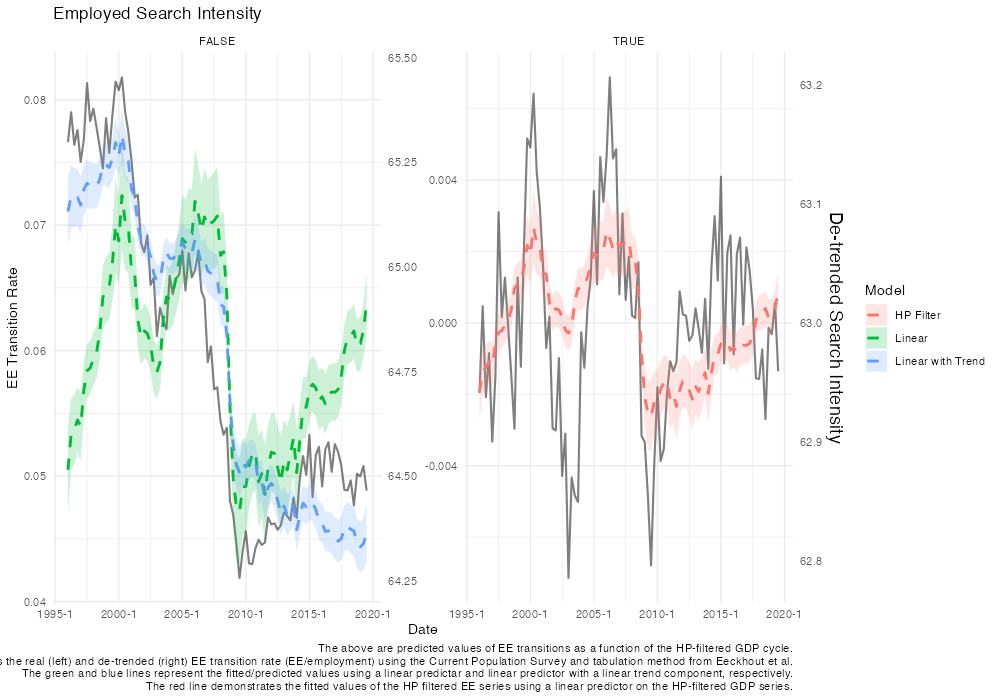
\includegraphics[keepaspectratio]{Eeckhout_Replication/emp_search_effort.png}}
\caption{Employed Search Effort Fit}
\end{figure}

\begin{verbatim}
##  [1] 0.2000000 0.2315789 0.2631579 0.2947368 0.3263158 0.3578947 0.3894737
##  [8] 0.4210526 0.4526316 0.4842105 0.5157895 0.5473684 0.5789474 0.6105263
## [15] 0.6421053 0.6736842 0.7052632 0.7368421 0.7684211 0.8000000
##  [1] 0.2000000 0.2315789 0.2631579 0.2947368 0.3263158 0.3578947 0.3894737
##  [8] 0.4210526 0.4526316 0.4842105 0.5157895 0.5473684 0.5789474 0.6105263
## [15] 0.6421053 0.6736842 0.7052632 0.7368421 0.7684211 0.8000000
\end{verbatim}

\begin{center}\includegraphics[width=0.9\linewidth]{behav_params_overview_files/figure-latex/unnamed-chunk-8-1} \end{center}

\begin{center}\includegraphics[width=0.9\linewidth]{behav_params_overview_files/figure-latex/unnamed-chunk-8-2} \end{center}

\begin{center}\includegraphics[width=0.9\linewidth]{behav_params_overview_files/figure-latex/unnamed-chunk-8-3} \end{center}

\begin{center}\includegraphics[width=0.9\linewidth]{behav_params_overview_files/figure-latex/unnamed-chunk-8-4} \end{center}

\begin{verbatim}
## 
## Call:
## lm(formula = as.formula(forms[which(names(forms) == form)]))
## 
## Residuals:
##       Min        1Q    Median        3Q       Max 
## -0.014882 -0.006066 -0.003639  0.007309  0.026123 
## 
## Coefficients:
##             Estimate Std. Error t value Pr(>|t|)    
## (Intercept) -0.17447    0.03519  -4.958 3.19e-06 ***
## x            0.23294    0.03499   6.656 1.93e-09 ***
## ---
## Signif. codes:  0 '***' 0.001 '**' 0.01 '*' 0.05 '.' 0.1 ' ' 1
## 
## Residual standard error: 0.01036 on 93 degrees of freedom
## Multiple R-squared:  0.3227, Adjusted R-squared:  0.3154 
## F-statistic: 44.31 on 1 and 93 DF,  p-value: 1.925e-09
## 
## 
## Call:
## lm(formula = as.formula(forms[which(names(forms) == form)]))
## 
## Residuals:
##        Min         1Q     Median         3Q        Max 
## -0.0102059 -0.0031620 -0.0001317  0.0039334  0.0079867 
## 
## Coefficients:
##               Estimate Std. Error t value Pr(>|t|)    
## (Intercept) -5.268e-02  1.773e-02  -2.970  0.00379 ** 
## x            1.285e-01  1.731e-02   7.423 5.61e-11 ***
## trend       -3.507e-04  1.918e-05 -18.285  < 2e-16 ***
## ---
## Signif. codes:  0 '***' 0.001 '**' 0.01 '*' 0.05 '.' 0.1 ' ' 1
## 
## Residual standard error: 0.004839 on 92 degrees of freedom
## Multiple R-squared:  0.8538, Adjusted R-squared:  0.8507 
## F-statistic: 268.7 on 2 and 92 DF,  p-value: < 2.2e-16
## 
## 
## Call:
## lm(formula = as.formula(forms[which(names(forms) == form)]))
## 
## Residuals:
##        Min         1Q     Median         3Q        Max 
## -0.0068610 -0.0016116  0.0001739  0.0018603  0.0046844 
## 
## Coefficients:
##              Estimate Std. Error t value Pr(>|t|)    
## (Intercept) -0.049270   0.008149  -6.046 3.05e-08 ***
## x            0.049021   0.008104   6.049 3.02e-08 ***
## ---
## Signif. codes:  0 '***' 0.001 '**' 0.01 '*' 0.05 '.' 0.1 ' ' 1
## 
## Residual standard error: 0.002399 on 93 degrees of freedom
## Multiple R-squared:  0.2824, Adjusted R-squared:  0.2747 
## F-statistic: 36.59 on 1 and 93 DF,  p-value: 3.018e-08
\end{verbatim}

\begin{center}\includegraphics[width=0.9\linewidth]{behav_params_overview_files/figure-latex/unnamed-chunk-8-5} \end{center}

\subsection{Learning Rate}\label{learning-rate}

\subsubsection{Mueller et al.~Job Seekers' Perceptions and Employment
Prospects: Heterogeneity, Duration Dependence and
Bias}\label{mueller-et-al.-job-seekers-perceptions-and-employment-prospects-heterogeneity-duration-dependence-and-bias}

\href{https://www.aeaweb.org/articles?id=10.1257/aer.20190808}{Mueller
et al: Job Seekers' Perceptions and Employment Prospects}

\emph{The authors claim to disentangle the effects of duration
dependence and dynamic selection by using job seekers' elicited beliefs
about job-finding. Assuming (and confirming empirically) that
job-seekers have realistic initial beliefs about job-finding they
isolate the heterogeneity in jobseekers from true duration dependence.
Ultimately, they find that dynamic selection selection explains most of
the negative duration dependence (rather than pure, true duration
dependence).}

\emph{Findings: Results are remarkably consistent even when including
additional data from 2019-2024.} The below results replicate the
findings in Mueller et al and extend the analysis to include a longer
time series. Plot and regression table titles have been maintained for
easy comparison.

We aim to include this information in our theoretical model of the job
search effort as a learning rate (ie. individuals learn about their
re-employment probability with repeated failures in the job search).

\begin{verbatim}
## 
## Descriptive Statistics (SCE)
## ===============================================================
## Variable                          Orig. 2013-19 2013-24 2020-24
## ---------------------------------------------------------------
## High-School Degree or Less            44.5       40.6    36.9  
## Some College Education                32.4       34.9    37.6  
## College Degree or More                23.1       24.6    25.6  
## Age 20-34                             25.4       27.2    30.0  
## Age 35-49                             33.5       33.6    35.3  
## Age 50-65                             41.1       39.2    34.8  
## Female                                59.3       61.2    60.8  
## Black                                 19.1       17.9    16.4  
## Hispanic                              12.5       13.0    12.6  
## UE transition rate                    18.7       19.1    18.2  
## UE transition rate: ST                25.8       26.5    24.3  
## UE transition rate: LT                12.7       12.7    12.3  
## # respondents                          948       1,367    433  
## # respondents w/ at least 2 u obs      534        780     252  
## # observations                        2,597      3,926   1,347 
## ---------------------------------------------------------------
\end{verbatim}

\begin{center}\includegraphics[width=0.9\linewidth]{behav_params_overview_files/figure-latex/unnamed-chunk-9-1} \end{center}

\begin{center}\includegraphics[width=0.9\linewidth]{behav_params_overview_files/figure-latex/unnamed-chunk-9-2} \end{center}

\begin{verbatim}
## [1] "Table 2—Regressions of Realized on Elicited 3-Month Job-Finding Probabilities (SCE)"
## [1] "Panel A. Contemporaneous elicitations"
\end{verbatim}

\begin{verbatim}
## 
## ========================================================================
##                                     Dependent variable:                 
##                     ----------------------------------------------------
##                                T+3 UE Transitions (3-Months)            
##                       Orig. 2013-19        2013-24          2020-24     
##                            (1)               (2)              (3)       
## ------------------------------------------------------------------------
## find_job_3mon           0.464***          0.396***          0.265***    
##                          (0.045)           (0.036)          (0.067)     
##                                                                         
## 1 | userid                                                              
##                                                                         
##                                                                         
## Constant                 -0.104            -0.080            -0.136     
##                          (0.169)           (0.137)          (0.267)     
##                                                                         
## ------------------------------------------------------------------------
## Observations              1,201             1,911             673       
## R2                        0.218             0.139            0.105      
## Adjusted R2               0.207             0.132            0.083      
## Residual Std. Error 0.467 (df = 1184) 0.475 (df = 1894) 0.478 (df = 656)
## ========================================================================
## Note:                                        *p<0.1; **p<0.05; ***p<0.01
\end{verbatim}

\begin{verbatim}
## 
## ==========================================================================
##                                       Dependent variable:                 
##                       ----------------------------------------------------
##                                  T+3 UE Transitions (3-Months)            
##                         Orig. 2013-19        2013-24          2020-24     
##                              (1)               (2)              (3)       
## --------------------------------------------------------------------------
## find_job_3mon             0.501***          0.418***          0.391***    
##                            (0.061)           (0.051)          (0.094)     
##                                                                           
## findjob_3mon_longterm     -0.258***         -0.170**         -0.360***    
##                            (0.088)           (0.071)          (0.133)     
##                                                                           
## longterm_unemployed        -0.078           -0.127***          -0.043     
##                            (0.051)           (0.041)          (0.075)     
##                                                                           
## 1 | userid                                                                
##                                                                           
##                                                                           
## Constant                   -0.062            -0.063            -0.402     
##                            (0.175)           (0.139)          (0.266)     
##                                                                           
## --------------------------------------------------------------------------
## Observations                1,201             1,911             673       
## R2                          0.259             0.182            0.155      
## Adjusted R2                 0.248             0.174            0.132      
## Residual Std. Error   0.455 (df = 1182) 0.464 (df = 1892) 0.465 (df = 654)
## ==========================================================================
## Note:                                          *p<0.1; **p<0.05; ***p<0.01
## [1] "Panel B. Lagged elicitations"
\end{verbatim}

\begin{verbatim}
## 
## ======================================================================
##                                    Dependent variable:                
##                     --------------------------------------------------
##                               T+3 UE Transitions (3-Months)           
##                      Orig. 2013-19       2013-24          2020-24     
##                           (1)              (2)              (3)       
## ----------------------------------------------------------------------
## tplus3_percep_3mon      0.332***         0.241***         0.203**     
##                         (0.067)          (0.056)          (0.102)     
##                                                                       
## 1 | userid                                                            
##                                                                       
##                                                                       
## Constant                 0.304           0.490**           0.451      
##                         (0.270)          (0.207)          (0.394)     
##                                                                       
## ----------------------------------------------------------------------
## Observations              474              798              300       
## R2                       0.168            0.090            0.179      
## Adjusted R2              0.139            0.071            0.132      
## Residual Std. Error 0.398 (df = 457) 0.436 (df = 781) 0.447 (df = 283)
## ======================================================================
## Note:                                      *p<0.1; **p<0.05; ***p<0.01
\end{verbatim}

\begin{verbatim}
## 
## ======================================================================
##                                    Dependent variable:                
##                     --------------------------------------------------
##                               T+3 UE Transitions (3-Months)           
##                      Orig. 2013-19       2013-24          2020-24     
##                           (1)              (2)              (3)       
## ----------------------------------------------------------------------
## find_job_3mon           0.301***         0.205***          -0.035     
##                         (0.069)          (0.058)          (0.110)     
##                                                                       
## 1 | userid                                                            
##                                                                       
##                                                                       
## Constant                 0.201           0.422**           0.361      
##                         (0.274)          (0.207)          (0.400)     
##                                                                       
## ----------------------------------------------------------------------
## Observations              474              798              300       
## R2                       0.159            0.083            0.168      
## Adjusted R2              0.129            0.064            0.121      
## Residual Std. Error 0.400 (df = 457) 0.437 (df = 781) 0.450 (df = 283)
## ======================================================================
## Note:                                      *p<0.1; **p<0.05; ***p<0.01
\end{verbatim}

\begin{center}\includegraphics[width=0.9\linewidth]{behav_params_overview_files/figure-latex/unnamed-chunk-9-3} \end{center}

\begin{center}\includegraphics[width=0.9\linewidth]{behav_params_overview_files/figure-latex/unnamed-chunk-9-4} \end{center}

\begin{verbatim}
## [1] "Table 4—Linear Regressions of Elicited Job-Finding Probabilities on Duration of Unemployment"
## +--------------------------------+----------+----------+----------+----------+
## |                                | (1)      | (2)      | (3)      | (4)      |
## +================================+==========+==========+==========+==========+
## | Orig. 2013-19                                                              |
## +--------------------------------+----------+----------+----------+----------+
## | Unemployment Duration (Months) | -0.0057  | -0.0050  | -0.0043  | 0.0022   |
## +--------------------------------+----------+----------+----------+----------+
## |                                | (0.0007) | (0.0007) | (0.0006) | (0.0049) |
## +--------------------------------+----------+----------+----------+----------+
## | Num.Obs.                       | 882      | 2281     | 2281     | 2281     |
## +--------------------------------+----------+----------+----------+----------+
## | R2                             | 0.110    | 0.090    | 0.155    | 0.824    |
## +--------------------------------+----------+----------+----------+----------+
## | 2013-24                                                                    |
## +--------------------------------+----------+----------+----------+----------+
## | Unemployment Duration (Months) | -0.0050  | -0.0048  | -0.0042  | -0.0026  |
## +--------------------------------+----------+----------+----------+----------+
## |                                | (0.0006) | (0.0006) | (0.0005) | (0.0034) |
## +--------------------------------+----------+----------+----------+----------+
## | Num.Obs.                       | 1265     | 3423     | 3399     | 3423     |
## +--------------------------------+----------+----------+----------+----------+
## | R2                             | 0.067    | 0.065    | 0.109    | 0.817    |
## +--------------------------------+----------+----------+----------+----------+
## | 2020-24                                                                    |
## +--------------------------------+----------+----------+----------+----------+
## | Unemployment Duration (Months) | -0.0011  | -0.0035  | -0.0039  | -0.0077  |
## +--------------------------------+----------+----------+----------+----------+
## |                                | (0.0013) | (0.0012) | (0.0013) | (0.0036) |
## +--------------------------------+----------+----------+----------+----------+
## | Num.Obs.                       | 395      | 1150     | 1140     | 1150     |
## +--------------------------------+----------+----------+----------+----------+
## | R2                             | 0.002    | 0.019    | 0.118    | 0.838    |
## +================================+==========+==========+==========+==========+
## | Standard errors are clustered at the user or spell level as indicated.     |
## +================================+==========+==========+==========+==========+
## Table: Table 4 - Panel A: Linear Regressions of Elicited Job-Finding Probabilities on Duration of Unemployment (SCE)
\end{verbatim}

\begin{center}\includegraphics[width=0.9\linewidth]{behav_params_overview_files/figure-latex/unnamed-chunk-9-5} \end{center}

\begin{center}\includegraphics[width=0.9\linewidth]{behav_params_overview_files/figure-latex/unnamed-chunk-9-6} \end{center}

\begin{center}\includegraphics[width=0.9\linewidth]{behav_params_overview_files/figure-latex/unnamed-chunk-9-7} \end{center}

\subsection{Additional Analyses}\label{additional-analyses}

\begin{enumerate}
\def\labelenumi{\arabic{enumi}.}
\tightlist
\item
  (Replicated with additional data for unemployed jobseekers)
  \href{https://www.aeaweb.org/articles?id=10.1257/mac.20160202}{\textbf{Mukoyama
  et al.~2018: Job Search Over the Business Cycle}}
\end{enumerate}

\emph{They provide a novel measure of job search effort exploiting the
American Time Use and Current Population Surveys which can be reduced to
just the intensive margin (changes in search effort by worker!). At the
moment, I think this will be the most useful input for our model.}

\emph{Abstract: We examine the cyclicality of search effort using
time-series, cross-state, and individual variation and find that it is
countercyclical. We then set up a search and matching model with
endogenous search effort and show that search effort does not amplify
labor market fluctuations but rather dampens them. Lastly, we examine
the role of search effort in driving recent unemployment dynamics and
show that the unemployment rate would have been 0.5 to 1 percentage
points higher in the 2008--2014 period had search effort not increased.}

\begin{enumerate}
\def\labelenumi{\arabic{enumi}.}
\setcounter{enumi}{3}
\tightlist
\item
  \textbf{Survey of Consumer Expectations Reservation Wages, Accepted
  Wages, and Wage Expectations} The data is unfortunately sparse and
  linking outcomes to reservation wages is difficult. However, in a
  cross-sectional setting we are able to deduce some weak relationships
  between Unemployment Duration and Absolute Reservation Wages and Wage
  Expectations.*
\end{enumerate}

\subsubsection{Reservation Wages}\label{reservation-wages}

Exploring the effect of unemployment duration on reservation wages,
accepted wages, and expected wage offers.

\textbf{Survey of Consumer Expectations Reservation Wages, Accepted
Wages, and Wage Expectations} (2014-2022) \emph{The data is
unfortunately sparse and linking outcomes to reservation wages is
difficult. However, in a cross-sectional setting we are able to deduce
some weak relationships between Unemployment Duration and Absolute
Reservation Wages and Wage Expectations.}

{[}1{]} ``Plots of RESERVATION WAGE versus latest, current wage''

\begin{center}\includegraphics[width=0.9\linewidth]{behav_params_overview_files/figure-latex/unnamed-chunk-10-1} \end{center}

\begin{center}\includegraphics[width=0.9\linewidth]{behav_params_overview_files/figure-latex/unnamed-chunk-10-2} \end{center}

{[}1{]} ``Plots of EXPECTED OFFER versus latest, current, reservation
wage''

\begin{center}\includegraphics[width=0.9\linewidth]{behav_params_overview_files/figure-latex/unnamed-chunk-10-3} \end{center}

{[}1{]} ``Plots of ACCEPTED SALARY versus latest, current, reservation
wage''

\begin{center}\includegraphics[width=0.9\linewidth]{behav_params_overview_files/figure-latex/unnamed-chunk-10-4} \end{center}

\begin{center}\includegraphics[width=0.9\linewidth]{behav_params_overview_files/figure-latex/unnamed-chunk-10-5} \end{center}

\begin{table}
\centering
\caption{\label{tab:unnamed-chunk-10}Accepted Wages and Unemployment Duration}
\centering
\begin{tabular}[t]{lcccccc}
\toprule
  & Accpt:Latest & AccptWage w.c & Accpt:ResWage & AccptWage:ResWage w.c & Accpt:EffResWage & AccptWage:EffResWage w.c\\
\midrule
(Intercept) & \num{0.826}*** & \num{1.743}*** & \num{0.933}*** & \num{1.199}*** & \num{0.826}*** & \num{1.002}***\\
 & (\num{0.108}) & (\num{0.260}) & (\num{0.045}) & (\num{0.141}) & (\num{0.051}) & (\num{0.177})\\
udur\_bins & \num{0.050} & \num{-0.005} & \num{-0.048}* & \num{-0.053}** & \num{0.008} & \num{-0.001}\\
 & (\num{0.045}) & (\num{0.048}) & (\num{0.019}) & (\num{0.020}) & (\num{0.023}) & (\num{0.024})\\
\midrule
Num.Obs. & \num{56} & \num{56} & \num{160} & \num{159} & \num{184} & \num{183}\\
R2 & \num{0.022} & \num{0.430} & \num{0.040} & \num{0.118} & \num{0.001} & \num{0.042}\\
RMSE & \num{0.40} & \num{0.35} & \num{0.30} & \num{0.30} & \num{0.34} & \num{0.34}\\
\bottomrule
\multicolumn{7}{l}{\rule{0pt}{1em}+ p $<$ 0.1, * p $<$ 0.05, ** p $<$ 0.01, *** p $<$ 0.001}\\
\end{tabular}
\end{table}
\begin{table}
\centering
\caption{\label{tab:unnamed-chunk-10}Reservation Wages and Unemployment Duration}
\centering
\begin{tabular}[t]{lcccc}
\toprule
  & ResWage & ResWage w.c & ResWage/LastWage & ResWage/LastWage w.c\\
\midrule
(Intercept) & \num{10.173}*** & \num{9.945}*** & \num{0.825}*** & \num{0.750}***\\
 & (\num{0.044}) & (\num{0.071}) & (\num{0.022}) & (\num{0.040})\\
udur\_bins & \num{0.107}*** & \num{0.083}*** & \num{0.027}*** & \num{0.023}***\\
 & (\num{0.012}) & (\num{0.011}) & (\num{0.006}) & (\num{0.006})\\
female &  & \num{-0.275}*** &  & \num{0.009}\\
 &  & (\num{0.022}) &  & (\num{0.012})\\
age &  & \num{0.005}*** &  & \num{0.001}*\\
 &  & (\num{0.001}) &  & (\num{0.000})\\
hhinc\_2 &  & \num{0.230}*** &  & \num{-0.008}\\
 &  & (\num{0.026}) &  & (\num{0.014})\\
hhinc\_3 &  & \num{0.427}*** &  & \num{-0.017}\\
 &  & (\num{0.030}) &  & (\num{0.017})\\
hhinc\_4 &  & \num{0.759}*** &  & \num{-0.008}\\
 &  & (\num{0.033}) &  & (\num{0.019})\\
education\_2 &  & \num{-0.247}*** &  & \num{0.050}+\\
 &  & (\num{0.045}) &  & (\num{0.026})\\
education\_3 &  & \num{-0.122}** &  & \num{0.007}\\
 &  & (\num{0.047}) &  & (\num{0.027})\\
education\_4 &  & \num{-0.046} &  & \num{0.052}+\\
 &  & (\num{0.051}) &  & (\num{0.029})\\
education\_5 &  & \num{0.027} &  & \num{0.008}\\
 &  & (\num{0.049}) &  & (\num{0.028})\\
education\_6 &  & \num{0.111}* &  & \num{0.054}+\\
 &  & (\num{0.054}) &  & (\num{0.031})\\
\midrule
Num.Obs. & \num{7937} & \num{7824} & \num{6294} & \num{6224}\\
R2 & \num{0.010} & \num{0.169} & \num{0.003} & \num{0.007}\\
R2 Adj. & \num{0.010} & \num{0.168} & \num{0.003} & \num{0.005}\\
AIC & \num{191435.4} & \num{187281.4} & \num{9054.4} & \num{8961.7}\\
BIC & \num{191456.4} & \num{187372.0} & \num{9074.6} & \num{9049.3}\\
Log.Lik. & \num{-11923.451} & \num{-11075.843} & \num{-4524.195} & \num{-4467.857}\\
RMSE & \num{0.98} & \num{0.90} & \num{0.44} & \num{0.44}\\
\bottomrule
\multicolumn{5}{l}{\rule{0pt}{1em}+ p $<$ 0.1, * p $<$ 0.05, ** p $<$ 0.01, *** p $<$ 0.001}\\
\end{tabular}
\end{table}
\begin{table}
\centering
\caption{\label{tab:unnamed-chunk-10}Accepted Wages and Unemployment Duration}
\centering
\begin{tabular}[t]{lcccc}
\toprule
  & AccptWage & AccptWage w.c & AccptWage/ResWage & AccptWage/ResWage w.c\\
\midrule
(Intercept) & \num{10.568}*** & \num{11.705}*** & \num{0.924}*** & \num{1.303}***\\
 & (\num{0.106}) & (\num{0.255}) & (\num{0.048}) & (\num{0.132})\\
udur\_bins & \num{-0.006} & \num{-0.037} & \num{-0.031}+ & \num{-0.036}+\\
 & (\num{0.040}) & (\num{0.037}) & (\num{0.018}) & (\num{0.018})\\
female &  & \num{-0.164} &  & \num{-0.073}\\
 &  & (\num{0.102}) &  & (\num{0.050})\\
age &  & \num{-0.008}* &  & \num{-0.005}**\\
 &  & (\num{0.004}) &  & (\num{0.002})\\
hhinc\_2 &  & \num{0.260}+ &  & \num{0.043}\\
 &  & (\num{0.139}) &  & (\num{0.067})\\
hhinc\_3 &  & \num{0.272}+ &  & \num{0.042}\\
 &  & (\num{0.138}) &  & (\num{0.069})\\
hhinc\_4 &  & \num{0.377}* &  & \num{-0.052}\\
 &  & (\num{0.150}) &  & (\num{0.075})\\
education\_2 &  & \num{-0.996}*** &  & \num{-0.043}\\
 &  & (\num{0.224}) &  & (\num{0.122})\\
education\_3 &  & \num{-0.940}*** &  & \num{-0.128}\\
 &  & (\num{0.223}) &  & (\num{0.122})\\
education\_4 &  & \num{-1.036}*** &  & \num{-0.176}\\
 &  & (\num{0.226}) &  & (\num{0.123})\\
education\_5 &  & \num{-0.827}*** &  & \num{-0.141}\\
 &  & (\num{0.224}) &  & (\num{0.124})\\
education\_6 &  & \num{-0.551}* &  & \num{-0.095}\\
 &  & (\num{0.228}) &  & (\num{0.127})\\
\midrule
Num.Obs. & \num{127} & \num{126} & \num{164} & \num{163}\\
R2 & \num{0.000} & \num{0.299} & \num{0.017} & \num{0.133}\\
R2 Adj. & \num{-0.008} & \num{0.232} & \num{0.011} & \num{0.070}\\
AIC & \num{2933.2} & \num{2884.9} & \num{110.6} & \num{109.9}\\
BIC & \num{2941.7} & \num{2921.7} & \num{119.9} & \num{150.1}\\
Log.Lik. & \num{-123.204} & \num{-99.911} & \num{-52.283} & \num{-41.957}\\
RMSE & \num{0.58} & \num{0.53} & \num{0.32} & \num{0.32}\\
\bottomrule
\multicolumn{5}{l}{\rule{0pt}{1em}+ p $<$ 0.1, * p $<$ 0.05, ** p $<$ 0.01, *** p $<$ 0.001}\\
\end{tabular}
\end{table}
\begin{table}
\centering
\caption{\label{tab:unnamed-chunk-10}Expected Wages and Unemployment Duration}
\centering
\begin{tabular}[t]{lcccc}
\toprule
  & ExpWage/ResWage & ExpWage/ResWage w.c & ExpWage/LastWage & ExpWage/LastWage w.c\\
\midrule
(Intercept) & \num{1.057}*** & \num{1.226}*** & \num{1.087}*** & \num{1.257}***\\
 & (\num{0.020}) & (\num{0.040}) & (\num{0.029}) & (\num{0.059})\\
udur\_bins & \num{-0.022}*** & \num{-0.009} & \num{-0.024}** & \num{-0.008}\\
 & (\num{0.006}) & (\num{0.006}) & (\num{0.008}) & (\num{0.009})\\
female &  & \num{-0.022}+ &  & \num{0.064}***\\
 &  & (\num{0.013}) &  & (\num{0.019})\\
age &  & \num{-0.003}*** &  & \num{-0.004}***\\
 &  & (\num{0.000}) &  & (\num{0.001})\\
hhinc\_2 &  & \num{0.004} &  & \num{-0.038}\\
 &  & (\num{0.016}) &  & (\num{0.023})\\
hhinc\_3 &  & \num{0.004} &  & \num{-0.001}\\
 &  & (\num{0.018}) &  & (\num{0.026})\\
hhinc\_4 &  & \num{0.000} &  & \num{-0.005}\\
 &  & (\num{0.019}) &  & (\num{0.027})\\
education\_2 &  & \num{-0.035} &  & \num{-0.032}\\
 &  & (\num{0.027}) &  & (\num{0.040})\\
education\_3 &  & \num{-0.008} &  & \num{-0.056}\\
 &  & (\num{0.028}) &  & (\num{0.041})\\
education\_4 &  & \num{0.004} &  & \num{-0.031}\\
 &  & (\num{0.030}) &  & (\num{0.044})\\
education\_5 &  & \num{0.011} &  & \num{-0.090}*\\
 &  & (\num{0.029}) &  & (\num{0.042})\\
education\_6 &  & \num{0.021} &  & \num{0.002}\\
 &  & (\num{0.032}) &  & (\num{0.046})\\
\midrule
Num.Obs. & \num{3114} & \num{3070} & \num{2721} & \num{2690}\\
R2 & \num{0.005} & \num{0.028} & \num{0.003} & \num{0.029}\\
R2 Adj. & \num{0.005} & \num{0.024} & \num{0.003} & \num{0.025}\\
AIC & \num{2803.9} & \num{2733.2} & \num{4079.4} & \num{3986.5}\\
BIC & \num{2822.1} & \num{2811.6} & \num{4097.2} & \num{4063.1}\\
Log.Lik. & \num{-1398.968} & \num{-1353.588} & \num{-2036.722} & \num{-1980.241}\\
RMSE & \num{0.34} & \num{0.34} & \num{0.46} & \num{0.45}\\
\bottomrule
\multicolumn{5}{l}{\rule{0pt}{1em}+ p $<$ 0.1, * p $<$ 0.05, ** p $<$ 0.01, *** p $<$ 0.001}\\
\end{tabular}
\end{table}

\subsubsection{Survey on Consumer Expectations - Job Search
Supplement}\label{survey-on-consumer-expectations---job-search-supplement}

The Federal Reserve Bank of New York compiles the nationally
representative Survey on Consumer Expectations annually in October.
Since 2013, they have run a Job Search Supplement which includes
questions on the time spent searching for work, and unemployment
duration. The job search supplement has plenty more questions that we
can look at incorporating, listed
\href{https://www.newyorkfed.org/medialibrary/Interactives/sce/sce/downloads/data/SCE-Labor-Market-Survey-Data-Codebook.pdf?sc_lang=en}{here}.
For now, I plot the relationship between time spent searching and time
out of work. The table below also indicates the number of people
unemployed in the dataset and the number of people unemployed and
searching.

\begin{longtable}[]{@{}rrr@{}}
\toprule\noalign{}
Year & N Unemployed & N Unemp \& Searching \\
\midrule\noalign{}
\endhead
\bottomrule\noalign{}
\endlastfoot
2014 & 383 & 70 \\
2015 & 321 & 44 \\
2016 & 339 & 46 \\
2017 & 350 & 38 \\
2018 & 354 & 41 \\
2019 & 343 & 32 \\
2020 & 304 & 45 \\
2021 & 330 & 50 \\
\end{longtable}

\begin{center}\includegraphics[width=0.9\linewidth]{behav_params_overview_files/figure-latex/unnamed-chunk-12-1} \end{center}

\begin{center}\includegraphics[width=0.9\linewidth]{behav_params_overview_files/figure-latex/unnamed-chunk-12-2} \end{center}

\subsubsection{On the job search}\label{on-the-job-search}

\begin{center}\includegraphics[width=0.9\linewidth]{behav_params_overview_files/figure-latex/unnamed-chunk-13-1} \end{center}

\end{document}
